\chapter{Orbital Optimization in Valence Bond Theory}
\label{chap_orbopt}

\ifthenelse{\boolean{wholethesis}}{\relax}{\begin{center}\textit{Generated on \today\ at \currenttime}\end{center}}

\noindent\textbf{Abstract:} The most time consuming step in optimizing a Valence Bond (VB) wave function is the construction of the matrix representation of the Hamilton operator ($\mathbf{H}$) and the corresponding overlap matrix ($\mathbf{S}$) for the wave function and the Brillouin states. In the 1990s a perturbation theory scheme, referred to as approximated Newton-Raphson (aNR), was introduced. For this scheme, not all $\mathbf{H}$ matrix elements need to be constructed. In this chapter an alternative, less time consuming method  to construct $\mathbf{H}$ matrix elements is introduced. In this method $\mathbf{H}$ matrix elements are replaced by elements of a Fock matrix.

\newpage

\section{Introduction}

\lettrine{\initial{I}}{}n 1916 Lewis suggested that atoms share electrons to form chemical bonds \cite{lewis}. Heitler and London incorporated this view a decade later into the quantum chemical description of the covalent bond in H$_2$ \cite{heitler}. In the 1930s Pauling used this description in his famous series of articles on ``The Nature Of The Chemical Bond'' \cite{pauling1,pauling2,pauling3,pauling4,pauling5,pauling6,pauling7,paulingbook}. This quantum chemical method is nowadays known as the Valence Bond theory.

In contrast to other methods, like the Molecular Orbital theory \cite{hartree1,hartree2,hartree3,fock} which uses delocalized doubly occupied orbitals by default, 
VB uses the spin-pairing of singly occupied non-orthogonal orbitals on different atoms, or molecular fragments to describe chemical bonds. The bond in H$_2$ can be described by the spin-coupling of the atomic $1s$ orbitals on both hydrogen atoms [H$\bullet$H$\bullet$]. The corresponding wave function consists of two determinants: $\Psi = |1s_{A}\overline{1s_{B}}| - |\overline{1s_{A}}1s_{B}|$. This determinant combination is called a structure. Since it describes the covalent character of the bond, it is referred to as the covalent structure. Ionic structures could be added to extend, or enhance the wave function: $|1s_{A}\overline{1s_{A}}|$ and $|1s_{B}\overline{1s_{B}}|$ (see Chapter \chintro). A VB wave function can be improved in two ways. Firstly, more structures can be added. A disadvantage in that case is that, when many structures are added, the interpretation of $\Psi$ becomes difficult. The second way to improve the wave function is the optimization of the orbitals. To maintain the interpretability, only a limited number of structures could be chosen of which the orbitals are optimized. 

Besides the use of multiple determinants in VB, non-orthogonal and localized orbitals are used explicitly. Since the orbitals in MO theory can be chosen to be orthogonal, this method attracted more attention. Its implementation in computer programs is more straightforward and computations on larger molecular systems are possible. Despite its computational hurdles, progress in Valence Bond theory continued \cite{vboverv1,vboverv2,vboverv3}. The main reason is the chemical interpretation of Valence Bond wave functions in term of structures. On the other hand several efficient methods to optimize Valence Bond wave functions, like Spin-Coupled Valence Bond (SCVB) \cite{scvb1,scvb2,scvb3} and Valence Bond Self-Consistent Field (VBSCF) \cite{vbscf1,vbscf2,koos1,zahid}, have been developed.

The most time consuming step in the optimization of the wave function is the optimization of the orbitals. Several optimization methods that compute the gradient of the total energy with respect to orbital rotations have been developed. The most common and widely applicable method is based on the evaluation of Hamiltonian matrix elements between Slater determinants, as introduced by L\"{o}wdin \cite{lowdin}. Despite its common applicability, this method is time consuming.

In another method, coined by Song \textit{et. al}, multiple Fock matrices are computed, one for each Slater determinant combination in the wave function \cite{song}. This approach is efficient and works fast for wave functions with a small number of Slater determinants. However, it is not as generally applicable as L\"{o}wdins method, because it cannot be used for wave functions containing orthogonal orbitals that are variably occupied, \textit{i.e.}, occur in some determinants, but not in all \cite{xmvb}. Although in VB non-orthogonal orbitals are used explicitly, orthogonality between the orbitals can occur.

In Multi Configurational Self-Consistent Field (MCSCF) \cite{joop,mcscf,roos1,roos2}, a method with similarities to VBSCF, elements of a common Fock matrix are used instead of Hamiltonian matrix elements computed via L\"{o}wdins formula \cite{roos1}. The central question for this chapter is whether it is also possible to use a single Fock matrix for the optimization of the orbitals in VBSCF, although those can be non-orthogonal. Rather than computing Hamiltonian matrix elements via the regular Slater-Condon rules \cite{koos3}, these elements might be, under conditions to be analyzed here, replaced by multiple elements from a single Fock matrix. This could save a considerable amount of computation time.

At first, the usability of Fock matrix elements instead of Hamiltonian matrix is analyzed by comparing the expression for Fock matrix elements with the expression for Hamiltonian matrix elements by L\"{o}wdin. Following this analysis, the implementation of these Fock matrix elements in TURTLE \cite{turtle}, the VB module in GAMESS-UK \cite{gamess}, will be presented. After the implementation details, speed-up factors of some test calculations will be discussed and compared. The chapter is concluded with an outlook on future enhancements.  

\section{Theory}

\subsection{\label{ch2.sec.vbsci}Valence Bond theory and Super CI}

To calculate the total energy of a molecular system, the time-independent Schr\"{o}dinger equation needs to be solved. The expectation value of the total energy for the system is:
\begin{equation}
E = \left< \Psi | \mathbf{H} | \Psi \right>,
\end{equation}
in which $\mathbf{H}$ is the Hamilton operator and $\Psi$ is the normalized wave function. A wave function is said to be optimized once the lowest possible value $E$ has been found. For Valence Bond theory, such a wave function $\Psi$ is constructed from a linear combination of structures:
\begin{equation}
\Psi = \sum_{i} C_i \Phi_i.
\label{ch2.eq.vbwf}
\end{equation}
These structures are linear combinations of Slater determinants:
\begin{equation}
\Phi = \sum_{i} \gamma_i \Delta_i,
\label{ch2.eq.struct}
\end{equation}
which are antisymmetrized products of spin-orbitals:
\begin{equation}
\Delta = |\chi_1\chi_2\chi_3\chi_4 \cdots \chi_n|,
\label{ch2.eq.determ}
\end{equation}
where the spin-orbitals $\chi$ have a spatial part ($\psi$) and a spin part which can be $\alpha$ or $\beta$. 
Orbitals $\psi$ are linear combinations of one electron basis functions:
\begin{equation}
\psi = \sum_{n} c_n \phi_n,
\label{ch2.eq.basis}
\end{equation}
in which the $c_n$ are orbital coefficients and $\phi_n$ one electron basis functions.

A Valence Bond wave function can be optimized by modifying the structure coefficients $C_i$ (equation \ref{ch2.eq.vbwf}) and the orbital coefficients $c_n$ (equation \ref{ch2.eq.basis}). Both optimizations can be performed simultaneously, as is done in a Newton-Raphson scheme \cite{zahid}, or sequentially with a method like Super CI \cite{superci1,superci2}. In Super CI, the structure coefficients $C_i$ are calculated first by solving the secular equation:
\begin{equation}
[\mathbf{H}-E\mathbf{S}] \cdot \mathbf{C} = 0,
\label{ch2.eq.eig}
\end{equation}
in which $\mathbf{H}$ and $\mathbf{S}$ are the Hamiltonian and overlap matrix in structure basis, respectively. Secondly, the orbitals are optimized, as will be explained below. After the orbital rotation step the secular equation \ref{ch2.eq.eig} is solved again with the new orbitals until both sets of coefficients no longer change.

The $\mathbf{H}$-matrix elements in equation \ref{ch2.eq.eig} are computed with L\"{o}wdins formula for each determinant combination in $\Psi$:
\begin{equation}
\begin{split}
\left< \Psi | \mathbf{H} | \Psi \right> &= \sum_{pq} C_p C_q \left< \Delta_p | \mathbf{H} | \Delta_q \right> \\ 
&= \sum_{pq} C_p C_q \left(\sum_{ik} h_{ik} \cdot S^{(i,k)} + \sum_{i<j,k<l} \left\{ \left[ \chi_i \chi_k | \chi_j \chi_l \right] - \left[ \chi_i \chi_l | \chi_j \chi_k \right] \right\} \cdot S^{(i,j,k,l)}\right),
\end{split}
\label{ch2.eq.lowdindeterminants}
\end{equation}
where $C_p$ and $C_q$ are determinant coefficients, $\Delta_p$ and $\Delta_q$ are determinants, $S^{(i,k)}$ and $S^{(i,j,k,l)}$ are first and second order cofactors\footnote{Cofactors are described in detail in Appendix A.}  and $h_{ik}$ and the term between curly brackets are one and two electron integrals, respectively.

Orbitals can be changed by adding a small amount of an other orbital. For instance, orbital $\psi_i$ can be changed by adding a small amount $\delta b_{ia}$ times $\psi_a$:
\begin{equation}
\psi_i' = \psi_i + \delta b_{ia} \psi_a.
\label{ch2.eq.orbchange}
\end{equation}
As a simple example, a single determinant wave function $\Psi_0=|\psi_i\overline{\psi_i}\psi_j\psi_k|$ with four orbitals is chosen. The orbital change of equation \ref{ch2.eq.orbchange} will result in:
\begin{equation}    
\begin{split}
|\psi_i'\overline{\psi_i'}\psi_j\psi_k | & = |(\psi_i + \delta b_{ia} \psi_a)\overline{(\psi_i + \delta b_{ia}\psi_a)}\psi_j\psi_k |\\
& = |\psi_i\overline{\psi_i}\psi_j\psi_k| + \delta b_{ia}|\psi_a\overline{\psi_i}\psi_j\psi_k| + \delta b_{ia} |\psi_i\overline{\psi_a}\psi_j\psi_k| + \delta b^2_{ia} |\psi_a\overline{\psi_a}\psi_j\psi_k|.\\
\end{split}
\label{ch2.eq.detchange}
\end{equation}
The first term is the original wave function $\Psi_0$. The second and third term are determinants, in which orbital $\psi_i$ has been replaced by $\psi_a$, once for $\alpha$ and once for $\beta$ spin. In the fourth determinant both occurrences of orbital $\psi_i$ have been replaced by $\psi_a$. This fourth determinant will be neglected here, because the amount $\delta b_{ia}$ is considered small and hence $\delta b_{ia}^2 \approx 0$.

The combination of the second and third determinant can be created from $|\psi_i\overline{\psi_i}\psi_j\psi_k |$ by the single excitation operator $\mathbf{C}_{i \rightarrow a}$, which replaces $\psi_i$ by $\psi_a$, once for $\alpha$ spin and once for $\beta$ spin \cite{ruttink}. This singly excited structure will be referred to as $\Psi_{ia}$. The change in $\Psi_0$ caused by the orbital change results (to first order) in:
\begin{equation}
\Psi_{0} \rightarrow \Psi_{0} + \delta b_{ia} \mathbf{C}_{i \rightarrow a} \Psi_{0} = \Psi_{0} + \delta b_{ia} \Psi_{ia}.
\label{ch2.eq.wfchange}
\end{equation}

With this mechanism orbital $\psi_i$ could be changed in such a way that the expectation value of the energy of $\Psi_0$ becomes lower. The minimum in the energy is found when the first order derivative of the energy with respect to the orbital change equals zero:
\begin{equation}
\frac{\partial E}{\partial b_{ia}}=\frac{\partial \frac{\left < \Psi_0 | \mathbf{H} | \Psi_0 \right >}{\left < \Psi_0 | \Psi_0 \right >}}{\partial b_{ia}}=0.
\label{ch2.eq.foderiv}
\end{equation}
Using the quotient rule, using the fact that $\left < \Psi_0 | \mathbf{H} | \Psi_0 \right >$ and $\left < \Psi_0 | \Psi_0 \right >$ are symmetric and using that the first order derivative with respect to the orbital change of $\Psi_0$ in equation \ref{ch2.eq.wfchange} equals $\Psi_{ia}$ \cite{vbscf2}, the first order derivative of the energy with respect to the orbital change can be written as: 
\begin{equation}
\begin{split}
\frac{\partial E}{\partial b_{ia}} & = \frac{2 \cdot \left < \Psi_0 | \mathbf{H} | \Psi_{ia} \right > \left< \Psi_0 | \Psi_0 \right > - 2 \cdot \left < \Psi_0 | \mathbf{H} | \Psi_0  \right > \left< \Psi_0 | \Psi_{ia}\right>}{\left < \Psi_0 | \Psi_0 \right > ^2 }\\
& = \frac{ 2 \cdot \left < \Psi_0 | \mathbf{H} | \Psi_{ia} \right > - 2 \cdot E_0 \left< \Psi_0 | \Psi_{ia} \right >}{\left < \Psi_0 | \Psi_0 \right >}\\
& = \frac{ 2 \cdot \left < \Psi_0 | \mathbf{H} - E_0 | \Psi_{ia} \right >}{\left < \Psi_0 | \Psi_0 \right >}.
\end{split}
\label{ch2.eq.foderiv2}
\end{equation}
For optimal orbitals, this first order derivative is equal to zero and hence:
\begin{equation}
\left < \Psi_0 | \mathbf{H} - E_0 | \Psi_{ia} \right > = 0.
\label{ch2.eq.brillouin}
\end{equation}
This is the Brillouin theorem, which states that with optimal orbitals singly excited states ($\Psi_{ia}$) do not interact or mix with the reference or ground state ($\Psi_0$) \cite{brillouin,genbrill}. 

In equations \ref{ch2.eq.orbchange}-\ref{ch2.eq.brillouin} the effect of a single orbital change has been shown. When all possible single excitations are taken into account, the wave function of equation \ref{ch2.eq.wfchange} can be written as:
\begin{equation}
\Psi_{superci} = \Psi_0 + \sum_{ia} b_{ia} \Psi_{ia},
\label{ch2.eq.superci}
\end{equation}
in which $\Psi_{superci}$ is the Super CI wave function, $i$ runs over all orbitals from which an excitation can be performed and $a$ runs over all orbitals to which excitations can take place. Values for $b_{ia}$ can be found by solving the generalized eigenvalue problem:
\begin{equation}
[\mathbf{H}-E_b\mathbf{S}] \cdot \mathbf{b} = 0,
\label{ch2.eq.geig}
\end{equation}
in which $\mathbf{H}$ and $\mathbf{S}$ are the Hamiltonian and metric in the basis of $\Psi_0$ and the singly excited states. $E_b$ is the lowest eigenvalue and $\mathbf{b}$ is the corresponding eigenvector. With the elements of $\mathbf{b}$ the orbitals are updated to make $\Psi_0$ equal to $\Psi_{superci}$ to first order:
\begin{equation}
\psi_i' = \psi_i + \sum_{a} b_{ia} \psi_a.
\label{ch2.eq.orbupd}
\end{equation}
With the modification of the orbitals the Super CI wave function is contracted or condensed into $\Psi_0$. This is exemplified for the change in orbital $\psi_i$ in the simple one determinant wave function in equation \ref{ch2.eq.detchange}. Orbital $\psi_i$ in $\Psi_0$ is modified with $\delta b_{ia}$ times orbital $\psi_a$, which results in determinant $|\psi_i'\overline{\psi_i'}\psi_j\psi_k |$:
\begin{equation}
\begin{split}
\Psi_{0} \leftarrow & \Psi_{0} + \delta b_{ia} \Psi_{ia} = \\
&|\psi_i\overline{\psi_i}\psi_j\psi_k| + \delta b_{ia}(|\psi_a\overline{\psi_i}\psi_j\psi_k| + |\psi_i\overline{\psi_a}\psi_j\psi_k|) \approx \\
&|(\psi_i + \delta b_{ia}\psi_a)\overline{(\psi_i + \delta b_{ia}\psi_a)}\psi_j\psi_k| = \\
&|\psi_i'\overline{\psi_i'}\psi_j\psi_k |.\\
\end{split}
\label{ch2.eq.condense}
\end{equation}
So, $\Psi_0$ will contain the updated orbital $\psi_i'$ which will be denoted $\psi_i$ in the next step (iteration). This procedure for a single orbital update is performed for all combinations in the summation in the Super CI wave function. Since the orbital changes are performed independently, they may be counteracting and therefore the Brillouin condition may not be fulfilled in a single step. Therefore, a new excitation pattern for a new $\Psi_{superci}$ is created. The eigenvalue problem is solved again and the orbitals are updated once more. It is expected that the orbital updates become smaller with each step. This procedure is repeated until all Brillouin elements, $\left < \Psi_0 | \mathbf{H} - E_0 | \Psi_{ia} \right >$, have become zero. At that point the expectation value of the energy ($E_0$) is stationary with respect to orbital changes (equation \ref{ch2.eq.foderiv2}).

Up till here, $\Psi_0$ was constructed of a single determinant, \textit{i.e.}, $|\psi_i\overline{\psi_i}\psi_j\psi_k|$. A regular VB wave function consists of multiple structures, and hence multiple determinants (see equations \ref{ch2.eq.vbwf} and \ref{ch2.eq.struct}). In that case, the contraction of equation \ref{ch2.eq.condense} will contain more determinants, all in which orbital $\psi_i$ has been replaced by $\psi_a$.

To solve the generalized eigenvalue problem of equation \ref{ch2.eq.geig}, both the Hamiltonian ($\mathbf{H}$) and the overlap ($\mathbf{S}$) are expressed in matrix form.  The Brillouin matrix is defined as the $\mathbf{H}$ matrix minus $E_0$ \cite{koos1}. Please note that for optimal orbitals, the Brillouin energy ($E_b$) in equation \ref{ch2.eq.geig} is equal to the energy of the ground state ($E_0$), because the singly exited states do no longer mix in with the ground state. 

An example of a Brillouin matrix is:
\begin{equation}
\left[\begin{array}{ccc}
\left< \Psi_{0} | \mathbf{H}-E_0 | \Psi_{0} \right> & \left< \Psi_{ia} | \mathbf{H}-E_0 | \Psi_{0} \right> & \left< \Psi_{ib} | \mathbf{H}-E_0 | \Psi_{0} \right> \\
\left< \Psi_{0} | \mathbf{H}-E_0 | \Psi_{ia} \right> & \left< \Psi_{ia} | \mathbf{H}-E_0 | \Psi_{ia} \right> & \left< \Psi_{ib} | \mathbf{H}-E_0 | \Psi_{ia} \right> \\
\left< \Psi_{0} | \mathbf{H}-E_0 | \Psi_{ib} \right> & \left< \Psi_{ia} | \mathbf{H}-E_0 | \Psi_{ib} \right> & \left< \Psi_{ib} | \mathbf{H}-E_0 | \Psi_{ib} \right> \\
\end{array}\right].
\label{ch2.eq.hamilt}
\end{equation}
This Brillouin matrix is constructed for a Super CI wave function that has two singly excitated states: $\Psi_{ia}$, for the excitation from orbital $\psi_i$ to $\psi_a$ and $\Psi_{ib}$, for the excitation from orbital $\psi_i$ to $\psi_b$. Brillouin matrices have the same dimension as the $\mathbf{H}$ and $\mathbf{S}$ matrices in equation \ref{ch2.eq.geig}. The calculation of the elements in $\mathbf{H}$ is expensive because of the large number of determinants, caused by the expansion into the Super CI wave function: for each excitation a Brillouin state, containing 1 to 2 times the number of determinants of $\Psi_0$, is added. For each determinant combination the evaluation of (large amounts of) subdeterminants \cite{koos2}, or cofactors are required.

To lower the computation time, Van Lenthe \textit{et al.} introduced a method, referred to as approximated Newton-Raphson (Section \ref{ch2.sec.anr}) \cite{koos1}, which requires less $\mathbf{H}$ and $\mathbf{S}$ matrix elements than regular Super CI \cite{koos1}, because elements of the type $\left < \Psi_{ia} | \mathbf{H} - E_0 | \Psi_{ib} \right >$ are not needed. This method will be explained in the next section.

\subsection{\label{ch2.sec.anr}The Approximated Newton-Raphson Method}

In the approximated Newton-Raphson technique perturbation theory is used to obtain orbital update coefficients. These coefficients are approximated by the quotient of the first column element and the diagonal element on each row of equation \ref{ch2.eq.hamilt}:
\begin{equation}
b_{ia}= - \frac{\left< \Psi_{0} | \mathbf{H}-E_0 | \Psi_{ia} \right>}{\left< \Psi_{ia} | \mathbf{H}-E_0 | \Psi_{ia} \right>}.
\label{ch2.eq.anr}
\end{equation}
This means that elements of the type $\left< \Psi_{ia} | \mathbf{H}-E_0 | \Psi_{ib} \right>$ are not used. In that way, only two matrix elements need to be calculated for such an excitation, instead of $m$, where $m$ equals the total number of excitations. This reduces the quadratic increase in number of matrix elements to linear.

Although the update coefficients $b_{ia}$ are calculated in a different way, the total energy $E_0$ will be the same. Once the orbitals are optimal the numerator in equation \ref{ch2.eq.anr} becomes zero and hence the Brillouin condition is fulfilled. 

A further reduction of the calculation time can be achieved if the numerator and the denominator in equation \ref{ch2.eq.anr} could be calculated, or approximated, faster. In the next section, the applicability of Fock matrix elements for the numerator and denominator in equation \ref{ch2.eq.anr} will be investigated.

\subsection{\label{ch2.sec.fock}Fock Matrix Elements} 

Roos \textit{et al.} showed that Brillouin matrix elements of the type $\left< \Psi_0 | \mathbf{H} | \Psi_{ia} \right>$ (the numerator in equation \ref{ch2.eq.anr}) could be replaced by elements of the Fock matrix ($F_{ia}$) for Complete Active Space Self-Consistent Field (CASSCF) wave functions \cite{roos1}. A CASSCF wave function is an MCSCF wave function for which all possible electron distributions in the variably occupied orbital space are included. The Fock matrix elements have the form:
\begin{equation}
F_{ia} = h_{ia} + \sum_{\sigma\nu} \left\{ \left[ \chi_i \chi_a | \chi_\sigma \chi_\nu \right] - \left[ \chi_i \chi_\nu | \chi_\sigma \chi_a \right] \right\} \cdot P^{(\sigma,\nu)},
\label{ch2.eq.fock}
\end{equation}
in which $F_{ia}$ is the Fock matrix element of spin-orbitals $\chi_i$ and $\chi_a$, $h_{ia}$ is the one electron integral $\left< \chi_i | \mathbf{h}| \chi_a \right>$. The double sum (over $\sigma$ and $\nu$) on the right hand side is over two electron integrals (Coulomb and exchange) times elements of the density matrix $P^{(\sigma,\nu)}$. This density matrix is constructed by adding up all contributions from first order reduced density matrices. Reduced density matrices are first order cofactors from the overlap determinants constructed for each determinant combination in $\Psi_0$. Examples to clarify the construction of the density matrix are given in equations \ref{ch2.eq.p0exampg}, \ref{ch2.eq.p0examp} and \ref{ch2.eq.p0examp2}.

In multideterminant wave functions, three orbital classes can be distinguished. The first class contains those orbitals that occur in all determinants. These will be denoted with labels $i$, $j$, $k$ and $l$. The second class contains orbitals that occur in some determinants, denoted with $t$, $u$, $v$ and $x$. The last class contains those orbitals that do not occur in the ground state wave function $\Psi_0$ and hence are virtual unoccupied orbitals, labeled $a$, $b$, $c$ and $d$. With those classes in mind, Roos \textit{et al.} published three expressions with Fock matrix elements for three types of excitations:
\begin{itemize}
\item{$i \rightarrow a$ from (always) doubly occupied to virtual orbitals}
\item{$t \rightarrow a$ from variably occupied to virtual orbitals}
\item{$i \rightarrow t$ from (always) doubly to variably occupied orbitals}
\end{itemize}
The fourth type of excitation, $t \rightarrow u$ from variably to variably occupied orbitals, is not needed in CASSCF, because all possible electron distributions in the variably occupied orbital space are already included in $\Psi_0$. In this section the applicability of Fock matrix elements in the construction of Brillouin matrix elements in VBSCF will be analyzed with L\"{o}wdins formula, equation \ref{ch2.eq.lowdindeterminants}. The difference between the one electron parts of L\"{o}wdins formula (equation \ref{ch2.eq.lowdindeterminants}) and the expression for a Fock matrix element (equation \ref{ch2.eq.fock}) is that in the former multiple one electron integrals are multiplied by first order cofactors ($S^{(i,k)}$), while in the latter only a single one electron integral occurs without a multiplication factor. Furthermore, the two electron integral part in the former is multiplied by second order cofactors ($S^{(i,j,k,l)}$), while in the latter those are multiplied by elements of the density matrix ($P^{(\sigma,\nu)}$). To analyze in which situations Fock matrix elements are equal to Brillouin matrix elements, a comparison of the cofactors in equation \ref{ch2.eq.lowdindeterminants} and the density matrix elements in equation \ref{ch2.eq.fock} is needed.

For this comparison the single determinant wave function $\Psi_0 = |\chi_1\chi_2\chi_3\chi_4\chi_5|$ is chosen. The excitation that will be examined for this wave function is from $\chi_1$ to $\chi_6$. Hence, $\Psi_{16}$ is equal to $|\chi_6\chi_2\chi_3\chi_4\chi_5|$. Numerals have been chosen as subscripts, rather than the previously specified letters: the classification of orbitals should not blur this comparison. 

In wave function $\Psi_0$, the orbitals $\chi$ are normalized, \textit{i.e.} $\left< \chi_1 | \chi_1 \right> = 1$. Throughout this chapter, normalized wave functions are used. This means that the determinants are multiplied by normalization constants in such a way that $\left< \Psi_0 |  \Psi_0 \right> = 1$:
\begin{equation}
\left < \Psi_0 | \Psi_0 \right> = | \mathbf{S} | = N^2 \cdot
\begin{array}{llllll}
 &  \chi_1 & \chi_2 & \chi_3 & \chi_4 & \chi_5 \\
 \chi_1 & \multicolumn{1}{|l}{ 1 } & s_{21} & s_{31} & s_{41} & \multicolumn{1}{l|}{ s_{51} } \\
 \chi_2 & \multicolumn{1}{|l}{ s_{12} } & 1 & s_{32} & s_{42} & \multicolumn{1}{l|}{ s_{52} } \\
 \chi_3 & \multicolumn{1}{|l}{ s_{13} } & s_{23} & 1 & s_{43} & \multicolumn{1}{l|}{ s_{53} } \\
 \chi_4 & \multicolumn{1}{|l}{ s_{14} } & s_{24} & s_{34} & 1 & \multicolumn{1}{l|}{ s_{54} } \\
 \chi_5 & \multicolumn{1}{|l}{ s_{15} } & s_{25} & s_{35} & s_{45} & \multicolumn{1}{l|}{ 1 }
\end{array} = 1,
\label{ch2.eq.s0g}
\end{equation}
in which the $s$ elements are overlaps between orbitals, for example, $s_{34} = \left< \chi_3 | \chi_4 \right>$. $N$ is the normalization constant\footnote{Throughout this chapter normalized wave functions are used. Therefore, the normalization constant $N$ is implicitly included.}. The density matrix, needed for the Fock matrix, is constructed from subdeterminants of this determinant. An example of a density matrix element is $P^{(3,4)}$:
\begin{equation}
P^{(3,4)}=
\begin{array}{llllll}
 & \hskip 53.0 pt \hbox{\lower 93pt\hbox{\vrule height100pt width 1.0pt}}\hskip-54.0pt \chi_1 & \chi_2 & \chi_3 & \chi_4 & \chi_5 \\
 \noalign{\vskip-91pt}
 \chi_1 & \multicolumn{1}{|l}{ 1 } & s_{21} & s_{31} & s_{41} & \multicolumn{1}{l|}{ s_{51} } \\
 \chi_2 & \multicolumn{1}{|l}{ s_{12} } & 1 & s_{32} & s_{42} & \multicolumn{1}{l|}{ s_{52} } \\
 \chi_3 & \multicolumn{1}{|l}{ s_{13} } & s_{23} & 1 & s_{43} & \multicolumn{1}{l|}{ s_{53} } \\
 \chi_4 & \multicolumn{1}{|l}{ s_{14} } & s_{24} & s_{34} & 1 & \multicolumn{1}{l|}{ s_{54} } \\
 \noalign{\vskip-8pt}
 \multispan6\hbox{\vrule  height 1.0 pt width140pt}\cr
 \noalign{\vskip 7pt}
 \chi_5 & \multicolumn{1}{|l}{ s_{15} } & s_{25} & s_{35} & s_{45} & \multicolumn{1}{l|}{ 1 }
\end{array} =
\begin{array}{lllll}
 &  \chi_1 & \chi_2 & \chi_4 & \chi_5 \\
 \chi_1 & \multicolumn{1}{|l}{ 1 } & s_{21} & s_{41} & \multicolumn{1}{l|}{ s_{51} } \\
 \chi_2 & \multicolumn{1}{|l}{ s_{12} } & 1 & s_{42} & \multicolumn{1}{l|}{ s_{52} } \\
 \chi_3 & \multicolumn{1}{|l}{ s_{13} } & s_{23} & s_{43} & \multicolumn{1}{l|}{s_{53}} \\
 \chi_5 & \multicolumn{1}{|l}{ s_{15} } & s_{25} & s_{45} & \multicolumn{1}{l|}{1}
\end{array},
\label{ch2.eq.p0exampg}
\end{equation}
which is the subdeterminant of $|\mathbf{S}|$ (equation \ref{ch2.eq.s0g}), from which the third column and the fourth row are removed.

First and second order cofactors that occur in equation \ref{ch2.eq.lowdindeterminants} are subdeterminants of the overlap determinant of $\Psi_0$ with $\Psi_{16}$:
\begin{equation}
\left < \Psi_0 | \Psi_{16} \right> =
\begin{array}{llllll}
 &  \chi_1 & \chi_2 & \chi_3 & \chi_4 & \chi_5 \\
 \chi_6 & \multicolumn{1}{|l}{ s_{16} } & s_{26} & s_{36} & s_{46} & \multicolumn{1}{l|}{ s_{56} } \\
 \chi_2 & \multicolumn{1}{|l}{ s_{12} } & 1 & s_{32} & s_{42} & \multicolumn{1}{l|}{ s_{52} } \\
 \chi_3 & \multicolumn{1}{|l}{ s_{13} } & s_{23} & 1 & s_{43} & \multicolumn{1}{l|}{ s_{53} } \\
 \chi_4 & \multicolumn{1}{|l}{ s_{14} } & s_{24} & s_{34} & 1 & \multicolumn{1}{l|}{ s_{54} } \\
 \chi_5 & \multicolumn{1}{|l}{ s_{15} } & s_{25} & s_{35} & s_{45} & \multicolumn{1}{l|}{ 1 }
\end{array}.
\label{ch2.eq.s016g}
\end{equation}
An example of a first order cofactor from $\left < \Psi_0 | \Psi_{16} \right>$ is $S^{(3,4)}$:
\begin{equation}
S^{(3,4)}=
\begin{array}{llllll}
 & \hskip 53.0 pt \hbox{\lower 93pt\hbox{\vrule height100pt width 1.0pt}}\hskip-54.0pt \chi_1 & \chi_2 & \chi_3 & \chi_4 & \chi_5 \\
 \noalign{\vskip-91pt}
 \chi_6 & \multicolumn{1}{|l}{ s_{16} } & s_{26} & s_{36} & s_{46} & \multicolumn{1}{l|}{ s_{56} } \\
 \chi_2 & \multicolumn{1}{|l}{ s_{12} } & 1 & s_{32} & s_{42} & \multicolumn{1}{l|}{ s_{52} } \\
 \chi_3 & \multicolumn{1}{|l}{ s_{13} } & s_{23} & 1 & s_{43} & \multicolumn{1}{l|}{ s_{53} } \\
 \chi_4 & \multicolumn{1}{|l}{ s_{14} } & s_{24} & s_{34} & 1 & \multicolumn{1}{l|}{ s_{54} } \\
 \noalign{\vskip-8pt}
 \multispan6\hbox{\vrule  height 1.0 pt width140pt}\cr
 \noalign{\vskip 7pt}
 \chi_5 & \multicolumn{1}{|l}{ s_{15} } & s_{25} & s_{35} & s_{45} & \multicolumn{1}{l|}{ 1 }
\end{array} =
\begin{array}{lllll}
 &  \chi_1 & \chi_2 & \chi_4 & \chi_5 \\
 \chi_6 & \multicolumn{1}{|l}{ s_{16} } & s_{26} & s_{46} & \multicolumn{1}{l|}{ s_{56} } \\
 \chi_2 & \multicolumn{1}{|l}{ s_{12} } & 1 & s_{42} & \multicolumn{1}{l|}{ s_{52} } \\
 \chi_3 & \multicolumn{1}{|l}{ s_{13} } & s_{23} & s_{43} & \multicolumn{1}{l|}{s_{53}} \\
 \chi_5 & \multicolumn{1}{|l}{ s_{15} } & s_{25} & s_{45} & \multicolumn{1}{l|}{1}
\end{array}.
\label{ch2.eq.s16g}
\end{equation}

On the first row in both determinants of equation \ref{ch2.eq.s16g} there are orbital overlaps, like $s_{26}$, which do not occur in the overlap determinant $\left< \Psi_0 | \Psi_0 \right>$. Brillouin matrix elements of the type $i \rightarrow t$ and $t \rightarrow u$ have first order cofactors like in equation \ref{ch2.eq.s016g}. Because these contain overlaps that do not occur in $\left< \Psi_0 | \Psi_0 \right>$, they are not equal to density matrix elements. Therefore, Brillouin matrix elements of the type $i \rightarrow t$ and $t \rightarrow u$ will be constructed the usual way via L\"{o}wdins formula (equation \ref{ch2.eq.lowdindeterminants}).

For the other types of excitations, $i \rightarrow a$ and $t \rightarrow a$, an electron is excited to a virtual orbital. In TURTLE, the virtual orbitals are chosen orthogonal to all other orbitals (see the Appendix of reference \cite{koos1}). If $\chi_6$ would be such a virtual orbital, the overlap of $\Psi_0$ with $\Psi_{16}$ becomes:
\begin{equation}
\left < \Psi_0 | \Psi_{16} \right> =
\begin{array}{llllll}
 &  \chi_1 & \chi_2 & \chi_3 & \chi_4 & \chi_5 \\
 \chi_6 & \multicolumn{1}{|l}{ 0 } & 0 & 0 & 0 & \multicolumn{1}{l|}{ 0 } \\
 \chi_2 & \multicolumn{1}{|l}{ s_{12} } & 1 & s_{32} & s_{42} & \multicolumn{1}{l|}{ s_{52} } \\
 \chi_3 & \multicolumn{1}{|l}{ s_{13} } & s_{23} & 1 & s_{43} & \multicolumn{1}{l|}{ s_{53} } \\
 \chi_4 & \multicolumn{1}{|l}{ s_{14} } & s_{24} & s_{34} & 1 & \multicolumn{1}{l|}{ s_{54} } \\
 \chi_5 & \multicolumn{1}{|l}{ s_{15} } & s_{25} & s_{35} & s_{45} & \multicolumn{1}{l|}{ 1 }
\end{array}.
\label{ch2.eq.s016go}
\end{equation}
With this orthogonality restriction, only 5 out of 25 possible cofactors would be non-zero. These 5 cofactors all have a corresponding $P$-matrix element, $P^{(n,1)}$. Whether it is possible to use these to construct Fock matrix elements for use in Brillouin matrix elements will be investigated.

\subsubsection{\label{ch2.sec.i-a}$i \rightarrow a$ from (always) doubly occupied to virtual orbitals}

To investigate the excitation type $i \rightarrow a$, the 5 electron wave function $|\chi_1\chi_2\chi_3\chi_4\chi_5|$ is changed into $|\chi_i\chi_j\chi_t\chi_u\chi_v|$, in which $\chi_i$ is $\psi_i$, $\chi_j$ is $\overline{\psi_i}$ and $\chi_t$, $\chi_u$ and $\chi_v$ are singly occupied orbitals. Spin for these orbitals is not specified and hence no attention needs to be paid to the spin integration in the overlap matrices that follow. Doubly occupied orbitals occur in all determinants and can be chosen orthogonal to all other orbitals \cite{koos1}. Although the 5 spin orbitals occur in ``all'' determinants in this single determinant wave function, $\chi_i$ and $\chi_j$ are chosen orthogonal to all other orbitals, while $\chi_t$, $\chi_u$ and $\chi_v$ are non-orthogonal to each other. Later on, the derivation for this single determinant wave function will be expanded for a multideterminant wave function in which orbitals $\chi_t$, $\chi_u$ and $\chi_v$ are variably occupied. The norm $\left < \Psi_0 | \Psi_0 \right>$ is the determinant of the overlap matrix, which will then have the following layout:
\begin{equation}
\left < \Psi_0 | \Psi_0 \right> = | \mathbf{S} | =
\begin{array}{llllll}
 &  \chi_i & \chi_j & \chi_t & \chi_u & \chi_v \\
 \chi_i & \multicolumn{1}{|l}{ 1 } & 0 & 0 & 0 & \multicolumn{1}{l|}{ 0 } \\
 \chi_j & \multicolumn{1}{|l}{ 0 } & 1 & 0 & 0 & \multicolumn{1}{l|}{ 0 } \\
 \chi_t & \multicolumn{1}{|l}{ 0 } & 0 & 1 & s_{ut} & \multicolumn{1}{l|}{s_{vt}} \\
 \chi_u & \multicolumn{1}{|l}{ 0 } & 0 & s_{tu} & 1 & \multicolumn{1}{l|}{s_{vu}} \\
 \chi_v & \multicolumn{1}{|l}{ 0 } & 0 & s_{tv} & s_{uv} & \multicolumn{1}{l|}{1}
\end{array}.
\label{ch2.eq.s0}
\end{equation}

In analogy with the example density matrix element in equation \ref{ch2.eq.p0exampg}, an example from density matrix element $P^{(t,u)}$, a cofactor of the norm in equation \ref{ch2.eq.s0}, is:
\begin{equation}
P^{(t,u)}=
\begin{array}{llllll}
 & \hskip 46.0 pt \hbox{\lower 93pt\hbox{\vrule height100pt width 1.0pt}}\hskip-47.0pt \chi_i & \chi_j & \chi_t & \chi_u & \chi_v \\
 \noalign{\vskip-91pt}
 \chi_i &  \multicolumn{1}{|l}{ 1 } & 0 & 0 & 0 & \multicolumn{1}{l|}{ 0 } \\
 \chi_j & \multicolumn{1}{|l}{ 0 } & 1 & 0 & 0 & \multicolumn{1}{l|}{ 0 } \\
 \chi_t & \multicolumn{1}{|l}{ 0 } & 0 & 1 & s_{ut} & \multicolumn{1}{l|}{s_{vt}} \\
 \chi_u & \multicolumn{1}{|l}{ 0 } & 0 & s_{tu} & 1 & \multicolumn{1}{l|}{s_{vu}} \\
 \noalign{\vskip-8pt}
 \multispan6\hbox{\vrule  height 1.0 pt width130pt}\cr
 \noalign{\vskip 7pt}
 \chi_v & \multicolumn{1}{|l}{ 0 } & 0 & s_{tv} & s_{uv} & \multicolumn{1}{l|}{ 1 }
\end{array} =
\begin{array}{lllll}
 &  \chi_i & \chi_j & \chi_u & \chi_v \\
 \chi_i & \multicolumn{1}{|l}{ 1 } & 0 & 0 & \multicolumn{1}{l|}{ 0 } \\
 \chi_j & \multicolumn{1}{|l}{ 0 } & 1 & 0 & \multicolumn{1}{l|}{ 0 } \\
 \chi_t & \multicolumn{1}{|l}{ 0 } & 0 & s_{ut} & \multicolumn{1}{l|}{s_{vt}} \\
 \chi_v & \multicolumn{1}{|l}{ 0 } & 0 & s_{uv} & \multicolumn{1}{l|}{1}
\end{array}.
\label{ch2.eq.p0examp}
\end{equation}

Since $\psi_i$ is doubly occupied, in $\chi_i$ and $\chi_j$, there are also two virtual orbitals for $\psi_a$, being $\chi_a \equiv \psi_a$ and $\chi_b \equiv \overline{\psi_a}$. The singly excited state wave function is $\Psi_{ia} = |\chi_a\chi_j\chi_t\chi_u\chi_v| + |\chi_i\chi_b\chi_t\chi_u\chi_v|$. These determinants will be referred to as $\Delta_{ia}$ and $\Delta_{jb}$, respectively. The overlap between $\Psi_0$, denoted here as $\Delta_0$, and both these determinants is:
\begin{equation}
\left < \Delta_0 | \Delta_{ia} \right > = 
\begin{array}{llllll}
 &  \chi_i & \chi_j & \chi_t & \chi_u & \chi_v \\
 \chi_a & \multicolumn{1}{|l}{ 0 } & 0 & 0 & 0 & \multicolumn{1}{l|}{ 0 } \\
 \chi_j & \multicolumn{1}{|l}{ 0 } & 1 & 0 & 0 & \multicolumn{1}{l|}{ 0 } \\
 \chi_t & \multicolumn{1}{|l}{ 0 } & 0 & 1 & s_{ut} & \multicolumn{1}{l|}{s_{vt}} \\
 \chi_u & \multicolumn{1}{|l}{ 0 } & 0 & s_{tu} & 1 & \multicolumn{1}{l|}{s_{vu}} \\
 \chi_v & \multicolumn{1}{|l}{ 0 } & 0 & s_{tv} & s_{uv} & \multicolumn{1}{l|}{1}
\end{array}
\label{ch2.eq.psi0_ia}
\end{equation}
and
\begin{equation}
\left < \Delta_0 | \Delta_{jb} \right > = 
\begin{array}{llllll}
 &  \chi_i & \chi_j & \chi_t & \chi_u & \chi_v \\
 \chi_i & \multicolumn{1}{|l}{ 1 } & 0 & 0 & 0 & \multicolumn{1}{l|}{ 0 } \\
 \chi_b & \multicolumn{1}{|l}{ 0 } & 0 & 0 & 0 & \multicolumn{1}{l|}{ 0 } \\
 \chi_t & \multicolumn{1}{|l}{ 0 } & 0 & 1 & s_{ut} & \multicolumn{1}{l|}{s_{vt}} \\
 \chi_u & \multicolumn{1}{|l}{ 0 } & 0 & s_{tu} & 1 & \multicolumn{1}{l|}{s_{vu}} \\
 \chi_v & \multicolumn{1}{|l}{ 0 } & 0 & s_{tv} & s_{uv} & \multicolumn{1}{l|}{1}
\end{array},
\label{ch2.eq.psi0_jb}
\end{equation}
which are both zero, because they contain a row and a column with zeroes.

To construct the Brillouin matrix element (equation \ref{ch2.eq.lowdindeterminants}), first and second order cofactors from the determinants in equations \ref{ch2.eq.psi0_ia} and \ref{ch2.eq.psi0_jb} are needed. Only two first order cofactors have a nonzero value, $S^{(i,a)}$ created by removing column $\chi_i$ and row $\chi_a$ from the determinant in equation \ref{ch2.eq.psi0_ia} and $S^{(j,b)}$ created by removing column $\chi_j$ and row $\chi_b$ from the determinant in equation \ref{ch2.eq.psi0_jb}. Other first order cofactors will be zero, because removing any other row or column will lead to a row or column with zeroes.

This means that per determinant combination only a single one electron integral contributes to the Brillouin matrix element, \textit{i.e.} $h_{ia} \cdot S^{(i,a)}$ and $h_{jb} \cdot S^{(j,b)}$. While the spin parts in $h_{ia}$ and $h_{jb}$ differ, $\chi_i$ and $\chi_a$ have $\alpha$ spin and $\chi_j$ and $\chi_b$ have $\beta$ spin, their spatial parts are equal. Furthermore, the first order cofactors, $S^{(i,a)}$ and $S^{(j,b)}$, and the norm (the determinant in equation \ref{ch2.eq.s0}) differ one unit in rank. The overlap determinant has a single ``1'' on the diagonal of the extra row and column and hence these cofactors are equal to the overlap determinant of the norm:
\begin{equation}
|\mathbf{S}| =
\begin{array}{llllll}
 &  \chi_i & \chi_j & \chi_t & \chi_u & \chi_v \\
 \chi_i & \multicolumn{1}{|l}{ 1 } & 0 & 0 & 0 & \multicolumn{1}{l|}{ 0 } \\
 \chi_j & \multicolumn{1}{|l}{ 0 } & 1 & 0 & 0 & \multicolumn{1}{l|}{ 0 } \\
 \chi_t & \multicolumn{1}{|l}{ 0 } & 0 & 1 & s_{ut} & \multicolumn{1}{l|}{s_{vt}} \\
 \chi_u & \multicolumn{1}{|l}{ 0 } & 0 & s_{tu} & 1 & \multicolumn{1}{l|}{s_{vu}} \\
 \chi_v & \multicolumn{1}{|l}{ 0 } & 0 & s_{tv} & s_{uv} & \multicolumn{1}{l|}{1}
\end{array}=
\begin{array}{lllll}
 &  \chi_j & \chi_t & \chi_u & \chi_v \\
 \chi_j & \multicolumn{1}{|l}{ 1 } & 0 & 0 & \multicolumn{1}{l|}{ 0 } \\
 \chi_t & \multicolumn{1}{|l}{ 0 } & 1 & s_{ut} & \multicolumn{1}{l|}{ s_{vt} } \\
 \chi_u & \multicolumn{1}{|l}{ 0 } & s_{tu} & 1 & \multicolumn{1}{l|}{s_{vu}} \\
 \chi_v & \multicolumn{1}{|l}{ 0 } & s_{tv} & s_{uv} & \multicolumn{1}{l|}{1}
\end{array}=
S^{(i,a)}=1,
\label{ch2.eq.sissia}
\end{equation}
and
\begin{equation}
S^{(i,a)}=
\begin{array}{lllll}
 &  \chi_j & \chi_t & \chi_u & \chi_v \\
 \chi_j & \multicolumn{1}{|l}{ 1 } & 0 & 0 & \multicolumn{1}{l|}{ 0 } \\
 \chi_t & \multicolumn{1}{|l}{ 0 } & 1 & s_{ut} & \multicolumn{1}{l|}{ s_{vt} } \\
 \chi_u & \multicolumn{1}{|l}{ 0 } & s_{tu} & 1 & \multicolumn{1}{l|}{s_{vu}} \\
 \chi_v & \multicolumn{1}{|l}{ 0 } & s_{tv} & s_{uv} & \multicolumn{1}{l|}{1}
\end{array}=
\begin{array}{lllll}
 &  \chi_i & \chi_t & \chi_u & \chi_v \\
 \chi_i & \multicolumn{1}{|l}{ 1 } & 0 & 0 & \multicolumn{1}{l|}{ 0 } \\
 \chi_t & \multicolumn{1}{|l}{ 0 } & 1 & s_{ut} & \multicolumn{1}{l|}{ s_{vt} } \\
 \chi_u & \multicolumn{1}{|l}{ 0 } & s_{tu} & 1 & \multicolumn{1}{l|}{s_{vu}} \\
 \chi_v & \multicolumn{1}{|l}{ 0 } & s_{tv} & s_{uv} & \multicolumn{1}{l|}{1}
\end{array}=
S^{(j,b)}=1.
\end{equation}
Since the wave function $\Psi_0$ is normalized, $|\mathbf{S}|$ (its norm) is equal to ``1''. Since  $S^{(i,a)}$ and $S^{(j,b)}$ are subdeterminants of $|\mathbf{S}|$ from which only a single ``1'' on the diagonal has been removed, these elements are also ``1''. The one electron contribution to the Brillouin matrix element is then: $h_{ia}\cdot S^{(i,a)} + h_{jb}\cdot S^{(j,b)} = 2 \cdot h_{ia}$.

The two electron integrals in equation \ref{ch2.eq.lowdindeterminants} are multiplied by second order cofactors. This means that besides removing column $\chi_i$ and row $\chi_a$ from the determinant in equation \ref{ch2.eq.psi0_ia} and column $\chi_j$ and row $\chi_b$ from the determinant in equation \ref{ch2.eq.psi0_jb}, another row and column need to be removed. Since index $i$ and $a$ (equation \ref{ch2.eq.psi0_ia}) and $j$ and $b$ (equation \ref{ch2.eq.psi0_jb}) are fixed, the summation in the two electron integral part of equation \ref{ch2.eq.lowdindeterminants} will only run over the other two indexes $\sigma$ and $\nu$:
\begin{equation}
\sum_{\sigma\nu} \left\{ [\chi_i\chi_a|\chi_\sigma\chi_\nu] - [\chi_i\chi_\nu|\chi_\sigma\chi_a] \right\} \cdot S^{(i,\sigma,a,\nu)},
\label{ch2.eq.twoel_ia}
\end{equation}
and
\begin{equation}
\sum_{\sigma\nu} \left\{ [\chi_j\chi_b|\chi_\sigma\chi_\nu] - [\chi_j\chi_\nu|\chi_\sigma\chi_b] \right\} \cdot S^{(j,\sigma,b,\nu)}.
\label{ch2.eq.twoel_jb}
\end{equation}
Because the operator in the two electron integral part, $\frac{1}{r_{12}}$, only operates on the spatial coordinates, the expressions in equations \ref{ch2.eq.twoel_ia} and \ref{ch2.eq.twoel_jb} are the same. Furthermore, second order cofactors $S^{(i,\sigma,a,\nu)}$ are equal to density matrix elements $P^{(\sigma,\nu)}$ (equation \ref{ch2.eq.p0examp}). A density matrix element is a determinant of which the rank is one unit higher than the rank of a second order cofactor. Like in the one electron part, this extra row and column have a ``1'' on the diagonal, while the rest of the column and row are zero. An example is the previously mentioned $P^{(t,u)}$ (equation \ref{ch2.eq.p0examp}) which is equal to $S^{(i,t,a,u)}$:
\begin{equation}
P^{(t,u)}=
\begin{array}{lllll}
 &  \chi_i & \chi_j & \chi_u & \chi_v \\
 \chi_i & \multicolumn{1}{|l}{ 1 } & 0 & 0 & \multicolumn{1}{l|}{ 0 } \\
 \chi_j & \multicolumn{1}{|l}{ 0 } & 1 & 0 & \multicolumn{1}{l|}{ 0 } \\
 \chi_t & \multicolumn{1}{|l}{ 0 } & 0 & s_{ut} & \multicolumn{1}{l|}{s_{vt}} \\
 \chi_v & \multicolumn{1}{|l}{ 0 } & 0 & s_{uv} & \multicolumn{1}{l|}{1}
\end{array}=
\begin{array}{llll}
 & \chi_j & \chi_u & \chi_v \\
 \chi_j & \multicolumn{1}{|l}{ 1 } & 0 & \multicolumn{1}{l|}{ 0 } \\
 \chi_t & \multicolumn{1}{|l}{ 0 } & s_{ut} & \multicolumn{1}{l|}{s_{vt}} \\
 \chi_v & \multicolumn{1}{|l}{ 0 } & s_{uv} & \multicolumn{1}{l|}{1}
\end{array}=S^{(i,t,a,u)}.
\end{equation}
With this, the total two electron integral contribution reduces to:
\begin{equation}
2 \cdot \sum_{\sigma\nu} \left\{ [\chi_i\chi_a|\chi_\sigma\chi_\nu] - [\chi_i\chi_\nu|\chi_\sigma\chi_a] \right\} \cdot P^{(\sigma,\nu)}.
\label{ch2.eq.twoel_ia_tot}
\end{equation}
Therefore, the total Brillouin matrix element is:
\begin{equation}
\begin{split}
\left < \Psi_0 | \mathbf{H} | \Psi_{ia} \right > & = 2 \cdot ( h_{ia} + \sum_{\sigma\nu} \left\{ [\chi_i\chi_a|\chi_\sigma\chi_\nu] - [\chi_i\chi_\nu|\chi_\sigma\chi_a] \right\} \cdot P^{(\sigma,\nu)}) \\
& = 2 \cdot F_{ia}.
\end{split}
\label{ch2.eq.brilisfock}
\end{equation}

Up till here only a single determinant wave function was used. A VB wave function consists of any number of determinants and therefore the derivation above will be expanded to multiple determinants.

A new VB wave function, consisting of one doubly occupied orbital $\psi_i$, expressed in spin-orbitals $\chi_i$ and $\chi_j$, and four partly occupied orbital, $\chi_t$, $\chi_u$, $\chi_v$ and $\chi_x$, is defined:
\begin{equation}
\Psi_0 = C_1 |\chi_i\chi_j\chi_t\chi_u|+ C_2 |\chi_i\chi_j\chi_v\chi_x|.
\label{ch2.eq.wfexamp2}
\end{equation}
The corresponding norm $\left< \Psi_0 | \Psi_0 \right>$ is:
\begin{equation}
\begin{split}
\left< \Psi_0 | \Psi_0 \right>=& C_1^2
\begin{array}{lllll}
 &  \chi_i & \chi_j & \chi_t & \chi_u \\
 \chi_i & \multicolumn{1}{|l}{ 1 } & 0 & 0 & \multicolumn{1}{l|}{ 0 } \\
 \chi_j & \multicolumn{1}{|l}{ 0 } & 1 & 0 & \multicolumn{1}{l|}{ 0 } \\
 \chi_t & \multicolumn{1}{|l}{ 0 } & 0 & 1 & \multicolumn{1}{l|}{s_{ut}} \\
 \chi_u & \multicolumn{1}{|l}{ 0 } & 0 & s_{tu} & \multicolumn{1}{l|}{1}
\end{array}+ C_1C_2
\begin{array}{lllll}
 &  \chi_i & \chi_j & \chi_t & \chi_u \\
 \chi_i & \multicolumn{1}{|l}{ 1 } & 0 & 0 & \multicolumn{1}{l|}{ 0 } \\
 \chi_j & \multicolumn{1}{|l}{ 0 } & 1 & 0 & \multicolumn{1}{l|}{ 0 } \\
 \chi_v & \multicolumn{1}{|l}{ 0 } & 0 & s_{tv} & \multicolumn{1}{l|}{s_{uv}} \\
 \chi_x & \multicolumn{1}{|l}{ 0 } & 0 & s_{tx} & \multicolumn{1}{l|}{s_{ux}}
\end{array} \\
& + C_2 C_1\begin{array}{lllll}
 &  \chi_i & \chi_j & \chi_v & \chi_x \\
 \chi_i & \multicolumn{1}{|l}{ 1 } & 0 & 0 & \multicolumn{1}{l|}{ 0 } \\
 \chi_j & \multicolumn{1}{|l}{ 0 } & 1 & 0 & \multicolumn{1}{l|}{ 0 } \\
 \chi_t & \multicolumn{1}{|l}{ 0 } & 0 & s_{vt} & \multicolumn{1}{l|}{s_{xt}} \\
 \chi_u & \multicolumn{1}{|l}{ 0 } & 0 & s_{vu} & \multicolumn{1}{l|}{s_{xu}}
\end{array}+ C_2^2
\begin{array}{lllll}
 &  \chi_i & \chi_j & \chi_v & \chi_x \\
 \chi_i & \multicolumn{1}{|l}{ 1 } & 0 & 0 & \multicolumn{1}{l|}{ 0 } \\
 \chi_j & \multicolumn{1}{|l}{ 0 } & 1 & 0 & \multicolumn{1}{l|}{ 0 } \\
 \chi_v & \multicolumn{1}{|l}{ 0 } & 0 & 1 & \multicolumn{1}{l|}{s_{xv}} \\
 \chi_x & \multicolumn{1}{|l}{ 0 } & 0 & s_{vx} & \multicolumn{1}{l|}{ 1 }
\end{array}.
\end{split}
\label{ch2.eq.s02}
\end{equation}

The density matrix is constructed by summing the contribution of the Slater determinant combinations in equation \ref{ch2.eq.s02}. If the row and column labels of the density matrix element are present in the Slater determinant combination, the corresponding is  added to the density matrix element. Since orbitals $\chi_i$ and $\chi_j$ occur in all determinants, density matrix elements $P^{(i,i)}$ and $P^{(j,j)}$ get a contribution from cofactors of all these determinants. Other elements get a contribution from less determinants, a single one in this case. For example $P^{(t,x)}$, which gets a single cofactor from the second determinant in equation \ref{ch2.eq.s02}:
\begin{equation}
P^{(t,x)}=
\begin{array}{llll}
 &  \chi_i & \chi_j & \chi_u \\
 \chi_i & \multicolumn{1}{|l}{ 1 } & 0 & \multicolumn{1}{l|}{ 0 } \\
 \chi_j & \multicolumn{1}{|l}{ 0 } & 1 & \multicolumn{1}{l|}{ 0 } \\
 \chi_v & \multicolumn{1}{|l}{ 0 } & 0 & \multicolumn{1}{l|}{ s_{uv} }
\end{array}.
\label{ch2.eq.p0examp2}
\end{equation} 

In the one determinant case it has been shown that the procedure for $\alpha$ and $\beta$ spin is the same. Therefore, only the excitation for the $\alpha$ spin electron will be analyzed here. A wave function $\Psi_{ia}$ is created by replacing all occurrences of $\chi_i$ by $\chi_a$:
\begin{equation}
\Psi_{ia} = C_1 |\chi_a\chi_j\chi_t\chi_u|+ C_2 |\chi_a\chi_j\chi_v\chi_x|.
\label{ch2.eq.psi_ia2}
\end{equation}

The overlap of $\Psi_0$ with $\Psi_{ia}$ is:
\begin{equation}
\begin{split}
\left<\Psi_0|\Psi_{ia} \right> =& C_1^2
\begin{array}{lllll}
 &  \chi_i & \chi_j & \chi_t & \chi_u \\
 \chi_a & \multicolumn{1}{|l}{ 0 } & 0 & 0 & \multicolumn{1}{l|}{ 0 } \\
 \chi_j & \multicolumn{1}{|l}{ 0 } & 1 & 0 & \multicolumn{1}{l|}{ 0 } \\
 \chi_t & \multicolumn{1}{|l}{ 0 } & 0 & 1 & \multicolumn{1}{l|}{s_{ut}} \\
 \chi_u & \multicolumn{1}{|l}{ 0 } & 0 & s_{tu} & \multicolumn{1}{l|}{1}
\end{array}+ C_1 C_2
\begin{array}{lllll}
 &  \chi_i & \chi_j & \chi_t & \chi_u \\
 \chi_a & \multicolumn{1}{|l}{ 0 } & 0 & 0 & \multicolumn{1}{l|}{ 0 } \\
 \chi_j & \multicolumn{1}{|l}{ 0 } & 1 & 0 & \multicolumn{1}{l|}{ 0 } \\
 \chi_v & \multicolumn{1}{|l}{ 0 } & 0 & s_{tv} & \multicolumn{1}{l|}{s_{uv}} \\
 \chi_x & \multicolumn{1}{|l}{ 0 } & 0 & s_{tx} & \multicolumn{1}{l|}{s_{ux}}
\end{array} \\
& + C_2 C_1 \begin{array}{lllll}
 &  \chi_i & \chi_j & \chi_v & \chi_x \\
 \chi_a & \multicolumn{1}{|l}{ 0 } & 0 & 0 & \multicolumn{1}{l|}{ 0 } \\
 \chi_j & \multicolumn{1}{|l}{ 0 } & 1 & 0 & \multicolumn{1}{l|}{ 0 } \\
 \chi_t & \multicolumn{1}{|l}{ 0 } & 0 & s_{vt} & \multicolumn{1}{l|}{s_{xt}} \\
 \chi_u & \multicolumn{1}{|l}{ 0 } & 0 & s_{vu} & \multicolumn{1}{l|}{s_{xu}}
\end{array}+ C_2^2
\begin{array}{lllll}
 &  \chi_i & \chi_j & \chi_v & \chi_x \\
 \chi_a & \multicolumn{1}{|l}{ 0 } & 0 & 0 & \multicolumn{1}{l|}{ 0 } \\
 \chi_j & \multicolumn{1}{|l}{ 0 } & 1 & 0 & \multicolumn{1}{l|}{ 0 } \\
 \chi_v & \multicolumn{1}{|l}{ 0 } & 0 & 1 & \multicolumn{1}{l|}{s_{xv}} \\
 \chi_x & \multicolumn{1}{|l}{ 0 } & 0 & s_{vx} & \multicolumn{1}{l|}{ 1 }
\end{array}.
\end{split}
\label{ch2.eq.psi0_ia2}
\end{equation}
The only one electron contribution that adds to the Brillouin matrix element is $h_{ia}$, because it is multiplied by nonzero  cofactors created by removing column $\chi_i$ and row $\chi_a$ from all four determinants in equation \ref{ch2.eq.psi0_ia2}. The sum of these four cofactors is equal to $\left< \Psi_0 | \Psi_0 \right>$ (equation \ref{ch2.eq.s02}). Since $\Psi_0$ is normalized, this is equal to one. The contribution is then, like for the one determinant case, $h_{ia}$ for $\alpha$ spin.

Only those two electron integrals that contain second order cofactors in which column $\chi_i$ and row $\chi_a$ are removed occur. One such combination of a Coulomb and exchange integral that contributes is: 
\begin{equation}
\left\{ [\chi_i\chi_a|\chi_t\chi_x] - [\chi_i\chi_x|\chi_t\chi_a] \right\} \cdot S_{12}^{(i,t,a,x)},
\label{ch2.eq.twoelexamp2}
\end{equation}
in which
\begin{equation}
S_{12}^{(i,t,a,x)}= 
\begin{array}{lll}
 &  \chi_j & \chi_u \\
 \chi_j & \multicolumn{1}{|l}{ 1 } & \multicolumn{1}{l|}{ 0 } \\
 \chi_v & \multicolumn{1}{|l}{ 0 } & \multicolumn{1}{l|}{ s_{uv} }
\end{array}=
\begin{array}{llll}
 &  \chi_i & \chi_j & \chi_u \\
 \chi_i & \multicolumn{1}{|l}{ 1 } & 0 & \multicolumn{1}{l|}{ 0 } \\
 \chi_j & \multicolumn{1}{|l}{ 0 } & 1 & \multicolumn{1}{l|}{ 0 } \\
 \chi_v & \multicolumn{1}{|l}{ 0 } & 0 & \multicolumn{1}{l|}{ s_{uv} }
\end{array}=
P^{(t,x)}.
\label{ch2.eq.cofac2isp2}
\end{equation}
If all contributing second order cofactors are taking into account, a double summation appears. Furthermore, the second order cofactors can be replaced by density matrix elements (equation \ref{ch2.eq.cofac2isp2}):
\begin{equation}
\sum_{\sigma\nu} \left\{ [\chi_i\chi_a|\chi_\sigma\chi_\nu] - [\chi_i\chi_\nu|\chi_\sigma\chi_a] \right\} \cdot P^{(\sigma,\nu)}.
\label{ch2.eq.twoel_ia_tot2}
\end{equation}

So, for the case with multiple determinants, the equality of equation \ref{ch2.eq.brilisfock} still holds:
\begin{equation}
\left<\Psi_0 | \mathbf{H} | \Psi_{ia} \right> = 2 \cdot F_{ia}.
\label{ch2.eq.fiafinal}
\end{equation}
Only a single one electron integral contributes to the Brillouin matrix element multiplied with one or more first order cofactors. Since these cofactors are equal to the determinants of the norm $\left< \Psi_0 | \Psi_0 \right>$, this factor will be ``1'' for a normalized wave function. For the two electron integral part, only Coulomb and exchange integrals in which $\chi_i$ and $\chi_a$ are present contribute. Furthermore, the second order cofactors are equal to density matrix elements, because the density matrix element will always have a single ``1'' on the diagonal of the extra row and column. This ``1'' arises from the fact that $\chi_i$ is orthogonal to all other orbitals.

\subsubsection{\label{ch2.sec.t-a}$t \rightarrow a$ from variably occupied to virtual orbitals}

For excitations of type $t \rightarrow a$, Roos \textit{et al.} have split the Fock matrix into an active and an inactive part \cite{roos1}. The total Fock matrix (equation \ref{ch2.eq.fock}) is the sum of these two parts:
\begin{equation}
F_{ia}=F^{I}_{ia} + F^{A}_{ia}.
\label{ch2.eq.focksum}
\end{equation}
In the inactive part the one electron contribution ($h_{ia}$) is present. Furthermore, the sum over the two electron integral runs over the inactive, or always occupied, orbitals:
\begin{equation}
F^{I}_{ia} = h_{ia} + \sum_{\lambda} \left\{ \left[ \chi_i \chi_a | \chi_\lambda \chi_\lambda \right] - \left[ \chi_i \chi_\lambda | \chi_\lambda \chi_a \right] \right\}.
\label{ch2.eq.focki}
\end{equation}
The two electron integral part is multiplied with $P^{(\lambda,\lambda)}$, which is equal to $\left<\Psi_0 | \Psi_0 \right> = 1$ (analogously to equation \ref{ch2.eq.sissia}: $P^{(i,i)}=S^{(i,a)}$). Therefore, these $P$-matrix elements are not shown in equation \ref{ch2.eq.focki}. 

The active part of the Fock matrix is constructed by summing over the two electron integral contribution for the variably occupied orbitals:
\begin{equation}
F^{A}_{ia} = \sum_{\sigma\nu} \left\{ \left[ \chi_i \chi_a | \chi_\sigma \chi_\nu \right] - \left[ \chi_i \chi_\nu | \chi_\sigma \chi_a \right] \right\} \cdot P^{(\sigma,\nu)}.
\label{ch2.eq.focka}
\end{equation}
It will be shown that the inactive part can be used in the construction of the Brillouin matrix element, while the active part cannot.

The wave function from the previous example $\Psi_0 = |\chi_i\chi_j\chi_t\chi_u\chi_v|$ is used here again, but this time the excitation is from orbital $\chi_t$ to $\chi_a$. In that case, $\left< \Psi_0 | \Psi_0 \right>$ will be the same as in equation \ref{ch2.eq.s0}, $\Psi_{ta}$ will be $|\chi_i\chi_j\chi_a\chi_u\chi_v|$ and the overlap of $\Psi_0$ with $\Psi_{ta}$ is:
\begin{equation}
\left < \Psi_0 | \Psi_{ta} \right > = 
\begin{array}{llllll}
 &  \chi_i & \chi_j & \chi_t & \chi_u & \chi_v \\
 \chi_i & \multicolumn{1}{|l}{ 1 } & 0 & 0 & 0 & \multicolumn{1}{l|}{ 0 } \\
 \chi_j & \multicolumn{1}{|l}{ 0 } & 1 & 0 & 0 & \multicolumn{1}{l|}{ 0 } \\
 \chi_a & \multicolumn{1}{|l}{ 0 } & 0 & 0 & 0 & \multicolumn{1}{l|}{ 0 } \\
 \chi_u & \multicolumn{1}{|l}{ 0 } & 0 & s_{tu} & 1 & \multicolumn{1}{l|}{s_{vu}} \\
 \chi_v & \multicolumn{1}{|l}{ 0 } & 0 & s_{tv} & s_{uv} & \multicolumn{1}{l|}{1}
\end{array}.
\label{ch2.eq.psi0_ta}
\end{equation}
Only those first order cofactors of the type $S^{(\sigma,a)}$ (with $\sigma$ being $t$, $u$, or $v$) contribute to the one electron contribution, other first order cofactors have a row with zeroes (labeled $\chi_a$). The total one electron contribution in L\"{o}wdins formula is:
\begin{equation}
h_{ta} \cdot S^{(t,a)} + h_{ua} \cdot S^{(u,a)} + h_{va} \cdot S^{(v,a)} = h_{ta} \cdot P^{(t,t)} + h_{ua} \cdot P^{(u,t)} + h_{va} \cdot P^{(v,t)},
\label{ch2.eq.ta_i1}
\end{equation}
using the fact that $P^{(\sigma,t)} = S^{(\sigma,a)}$, for $\sigma$ is $t$, $u$ and $v$.

The two electron contribution can be split into two parts. The first part contains the second order cofactors for which the first index $\sigma$ runs over the variably occupied orbitals and the second and fourth index run over $\lambda$, the doubly occupied space. The third index is $a$, because second order cofactors without $a$ will be zero, because those are determinants with a row of zeroes. With the selection of an orthogonal occupied orbital for the second index, like $i$, only the selection of $i$ as fourth index will result in a non-zero second order cofactor. An example is $S^{(t,i,a,i)}$. Removing the column and row labeled $i$ results in removing a single ``1'' from the diagonal of the determinant and hence $S^{(t,i,a,i)}=S^{(t,a)}=P^{(t,t)}$:
\begin{equation}
S^{(t,i,a,i)}=
\begin{array}{llll}
 &  \chi_j & \chi_u & \chi_v \\
 \chi_j & \multicolumn{1}{|l}{ 1 } & 0 & \multicolumn{1}{l|}{ 0 } \\
 \chi_u & \multicolumn{1}{|l}{ 0 } & 1 & \multicolumn{1}{l|}{s_{vu}} \\
 \chi_v & \multicolumn{1}{|l}{ 0 } & s_{uv} & \multicolumn{1}{l|}{1}
\end{array}=
\begin{array}{lllll}
 &  \chi_i & \chi_j & \chi_u & \chi_v \\
 \chi_i & \multicolumn{1}{|l}{ 1 } & 0 & 0 & \multicolumn{1}{l|}{ 0 } \\
 \chi_j & \multicolumn{1}{|l}{ 0 } & 1 & 0 & \multicolumn{1}{l|}{ 0 } \\
 \chi_u & \multicolumn{1}{|l}{ 0 } & 0 & 1 & \multicolumn{1}{l|}{s_{vu}} \\
 \chi_v & \multicolumn{1}{|l}{ 0 } & 0 & s_{uv} & \multicolumn{1}{l|}{1}
\end{array}=
S^{(t,a)}=P^{(t,t)}.
\label{ch2.eq.stiai-sta}
\end{equation}
The two electron contribution for $\lambda = i$ is then:
\begin{equation}
\begin{split}
&\left\{ \left[ \chi_t \chi_a | \chi_i \chi_i \right] - \left[ \chi_t \chi_i | \chi_i \chi_a \right] \right\} \cdot P^{(t,t)}\\
+&\left\{ \left[ \chi_u \chi_a | \chi_i \chi_i \right] - \left[ \chi_u \chi_i | \chi_i \chi_a \right] \right\} \cdot P^{(u,t)}\\
+&\left\{ \left[ \chi_v \chi_a | \chi_i \chi_i \right] - \left[ \chi_v \chi_i | \chi_i \chi_a \right] \right\} \cdot P^{(v,t)},
\end{split}
\label{ch2.eq.ta_i2}
\end{equation} 
and analogously for $\lambda = j$:
\begin{equation}
\begin{split}
&\left\{ \left[ \chi_t \chi_a | \chi_j \chi_j \right] - \left[ \chi_t \chi_j | \chi_j \chi_a \right] \right\} \cdot P^{(t,t)}\\
+&\left\{ \left[ \chi_u \chi_a | \chi_j \chi_j \right] - \left[ \chi_u \chi_j | \chi_j \chi_a \right] \right\} \cdot P^{(u,t)}\\
+&\left\{ \left[ \chi_v \chi_a | \chi_j \chi_j \right] - \left[ \chi_v \chi_j | \chi_j \chi_a \right] \right\} \cdot P^{(v,t)}.
\end{split}
\label{ch2.eq.ta_i3}
\end{equation}
Summing up the contributions from equations \ref{ch2.eq.ta_i1}, \ref{ch2.eq.ta_i2} and \ref{ch2.eq.ta_i3}, one finds the ``inactive'' contribution to the Brillouin matrix element to be:
\begin{equation}
F^{I}_{ta} \cdot P^{(t,t)} + F^{I}_{ua} \cdot P^{(u,t)} + F^{I}_{va} \cdot P^{(v,t)}.
\label{ch2.eq.ta_i4}
\end{equation}

The second part of the two electron integrals contains the second order cofactors of the type $S^{(\sigma,\mu,a,\nu)}$, with $\sigma$, $\mu$ and $\nu$ being $t$, $u$ or $v$. For these second order cofactors no equivalent $P$-matrix element is present. Therefore, the contribution to the Brillouin matrix element from this second part of the two electron integrals is:
\begin{equation}
\sum_{\sigma,\mu,\nu} \left\{ \left[ \chi_\sigma \chi_a | \chi_\mu \chi_\nu \right] - \left[ \chi_\sigma \chi_\nu | \chi_\mu \chi_a \right] \right\} \cdot S^{(\sigma,a,\mu,\nu)},
\label{ch2.eq.ta_i5}
\end{equation}
in which $\sigma$, $\mu$ and $\nu$ only run over the variably occupied, or active, orbital space.

The Brillouin matrix element $\left< \Psi_0 | \mathbf{H} | \Psi_{ta} \right>$ is the sum of the contributions in equations \ref{ch2.eq.ta_i4} and \ref{ch2.eq.ta_i5}:
\begin{equation}
\left< \Psi_0 | \mathbf{H} | \Psi_{ta} \right> = \sum_{\sigma} F^{I}_{t\sigma} \cdot P^{(\sigma,t)} + \sum_{\sigma,\mu,\nu} \left\{ \left[ \chi_\sigma \chi_a | \chi_\mu \chi_\nu \right] - \left[ \chi_\sigma \chi_\nu | \chi_\mu \chi_a \right] \right\} \cdot S^{(\sigma,a,\mu,\nu)}.
\label{ch2.eq.ta_i6}
\end{equation}

Up till here, only a single determinant wave function has been used for showing the usability of multiple Fock matrix elements for a single Brillouin matrix element of the type $t \rightarrow a$. If multiple determinants would be used, it will become clear that the density matrix elements become sums of contributions for each determinant combination, analogously to equations \ref{ch2.eq.wfexamp2} to \ref{ch2.eq.psi0_ia2}. Since the $P$-matrix element already contains the sums over the determinants, only the second part in equation \ref{ch2.eq.ta_i6} get an extra summation over the Slater determinants in $\Psi_0$ and $\Psi_{ta}$:
\begin{equation}
\left< \Psi_0 | \mathbf{H} | \Psi_{ta} \right> = \sum_{\sigma} F^{I}_{t\sigma} \cdot P^{(\sigma,t)} + \sum_{pq} C_p C_q\sum_{\sigma,\mu,\nu} \left\{ \left[ \chi_\sigma \chi_a | \chi_\mu \chi_\nu \right] - \left[ \chi_\sigma \chi_\nu | \chi_\mu \chi_a \right] \right\} \cdot S_{pq}^{(\sigma,a,\mu,\nu)},
\label{ch2.eq.ta_i7}
\end{equation}
in which $C_p$ and $C_q$ are the determinant coefficients in $\Psi_0$ and $\Psi_{ta}$, respectively. 

Comparing equation \ref{ch2.eq.fiafinal} for $i \rightarrow a$ with equation \ref{ch2.eq.ta_i7} for $t \rightarrow a$, one immediately sees the big difference in complexity. Using equation \ref{ch2.eq.fiafinal}, only a single Fock matrix element can be used instead of the Brillouin matrix element. Unfortunately, using equation \ref{ch2.eq.ta_i7} it becomes clear that the Fock matrix needs to be split into an inactive and an active part, a series of inactive Fock matrix elements is needed and a sum over two electron integrals multiplied with second order cofactors are necessary.

\subsubsection{\label{ch2.sec.delocal}Localized VB wave functions}

In TURTLE, it is possible to restrict orbitals to certain atoms, or fragments of the molecule. This type of wave function is called localized. Within each fragment, the doubly occupied and virtual orbitals are orthogonal to all other orbitals. However, between fragments, overlap of orbitals can occur. This means that doubly occupied orbitals from one fragment are no longer necessarily orthogonal to the orbitals in another fragment. Overlaps between orbitals on different fragments will not be zero and hence density matrix elements in the Fock matrix elements (equation \ref{ch2.eq.fock}) are not equal to the second order cofactors in L\"{o}wdins formula (equation \ref{ch2.eq.lowdindeterminants}): the required single ``1'' on the extra row and column of the density matrix is not present. Therefore, the reasoning in the previous section for excitations of the types $i \rightarrow a$ and $t \rightarrow a$ does not apply for localized VB wave functions. 

Sometimes, however, orbitals from different fragments can still be orthogonal due to the symmetry in the molecule (see the examples in Section \ref{ch2.sec.aromat}). In that case the elements of the Fock matrix can be used instead of calculating the Brillouin matrix elements.

\subsubsection{\label{ch2.sec.denominator}Approximation Of The Denominator}

So far, the numerator of equation \ref{ch2.eq.anr} has been analyzed. The denomator contains elements of the type $\left< \Psi_{ia} | \mathbf{H}-E_0 | \Psi_{ia} \right>$. These correspond to the energy of the singly excited states. This energy can be approximated as the ground state energy ($E_0$) minus the energy of the orbital from which the excitation takes place ($F_{ii}$) plus the energy of the orbital to which the excitation takes place ($F_{aa}$):
\begin{equation}
\left< \Psi_{ia} | \mathbf{H}-E_0 | \Psi_{ia} \right> \approx (E_0 - F_{ii} + F_{aa})\left< \Psi_{ia} | \Psi_{ia} \right>.
\label{ch2.eq.cheapdiag}
\end{equation}
This is an approximation, since removing an orbital will influence other orbitals, which is not taken into account here. An advantage of approximating the diagonal Brillouin matrix element with the difference of two Fock matrix elements is that it saves time, especially when the wave function consists of a lot of determinants. On the other hand, the orbital update coefficients will be less accurate because of this approximation. It can therefore not be predicted how this approximation will affect the optimization process and the computation time.

\section{\label{ch2.sec.implementation}Implementation}

The implementation of the approximations described in the previous section consists of two parts. Firstly, the approximated Newton-Raphson method, which was already implemented in TURTLE, has been extended with extra options. Secondly, the use of a Fock matrix for excitations from doubly occupied orbitals to virtuals (equation \ref{ch2.eq.fiafinal}) has been implemented from scratch. It was decided not to implement equation \ref{ch2.eq.ta_i7} for excitations from variably occupied to virtuals, because the number of excitations from $t$ to $a$ is in most cases much lower than the number of excitations from $i$ to $a$. Moreover, Brillouin matrix elements for $t \rightarrow a$ with their series of inactive Fock matrix elements and second order cofactors are much more time consuming to construct than Brillouin matrix elements for $i \rightarrow a$, which consist only of the single Fock matrix element $F_{ia}$.

In the original aNR implementation the perturbation (equation \ref{ch2.eq.anr}) was used for excitations from the always and partly occupied orbitals to the virtuals. For all other excitations, \textit{i.e.} those from the always occupied orbitals to the partly occupied orbitals and from partly occupied to other partly occupied orbitals, an $\mathbf{H}$ and $\mathbf{S}$ matrix were constructed, for which the update coefficients were retrieved by solving the generalized eigenvalue problem (equation \ref{ch2.eq.geig}). 

In the current implementation there are three optimization options per excitation. The first option is that the excitation is treated with Super CI. In that case all interaction elements will be calculated. These are the interaction element of the ground state with the singly excited state, like $\left < \Psi_{0} | \mathbf{H} - E_0 | \Psi_{ia} \right >$, the diagonal element, $\left < \Psi_{ia} | \mathbf{H} - E_0 | \Psi_{ia} \right >$, and all interaction elements with other singly excited structures, like $\left < \Psi_{ia} | \mathbf{H} - E_0 | \Psi_{ib} \right >$. Please note, that these latter elements are only calculated when both excitations ($i \rightarrow a$ and $i \rightarrow b$) are treated with Super CI.

The second option is that the excitation is treated with approximated Newton-Raphson. In that case only the two matrix elements in equation \ref{ch2.eq.anr} are calculated to obtain the update coefficient $b_{ia}$.

In the third option the excitation is treated with the Fock operator. In that case the orbital update coefficient $b_{ia}$ is calculated by dividing the Fock matrix element of the type $F_{ia}$ by the difference between $F_{ii}$ and $F_{aa}$ (Section \ref{ch2.sec.denominator}):
\begin{equation}
b_{ia}= - \frac{2 \cdot F_{ia}}{E_0 - F_{ii} + F_{aa}}.
\label{ch2.eq.fockapprox}
\end{equation}

For excitations treated with regular Super CI, the $\mathbf{b}$ vector is calculated by solving the generalized eigenvalue problem (equation \ref{ch2.eq.geig}). This eigenvector is subsequently padded with the separately calculated update coefficients of equations \ref{ch2.eq.anr} and \ref{ch2.eq.fockapprox}. With the elements of this $\mathbf{b}$ vector the orbitals are updated, like in equation \ref{ch2.eq.condense}.

The three options above suggest that the user needs to specify beforehand which Brillouin matrix rows (or excitations) should be treated with which option. Since the virtual space is not yet created at the beginning of the calculation it is not very practical to specify the optimization method per excitation. Therefore, two additional specification options have been added: the specification per occupied orbital and the specification per orbital class. All excitations for either a certain orbital or all orbitals in a class are treated with the same option, be-it \textit{superci}, \textit{pert} or the new \textit{fock}.

It should be noted that the \textit{fock} option can only be used for the optimization of orbitals which are orthogonal to all other orbitals. The most commonly used specification option, at least for the calculations reported in this thesis, is the specification per orbital class. 

\section{Sample Calculations}

In this section results from a few test calculations will be presented. The calculations have been run on an SGI Origin 2000 with R12000 processors. In the first example results from several calculations with the \textit{superci}, the \textit{pert} and the new \textit{fock} option are compared.  In the second example some of the new parameters for the extended \textit{pert} option are tested. The results are compared to those from a complete Super CI calculation.

\subsection{\label{ch2.sec.aromat}First Example: Cyclic Hydrocarbons}

Aromaticity has been and still is widely studied using Valence Bond theory \cite{cooper1,cooper2,remcolowdin,indacene,fowler,jenneskens,cyclohexatriene,bestbenzene,benzyne}. The molecules involved are planar, having a strict separation of the $\sigma$ and $\pi$ system. For the test four planar molecules, cyclobutadiene (\textbf{1}), benzene (\textbf{2}), cyclooctatetraene (\textbf{3}) and pentalene (\textbf{4}) have been selected (Figure \ref{ch2.fig.compounds}).
\begin{figure}[htdp]
\center
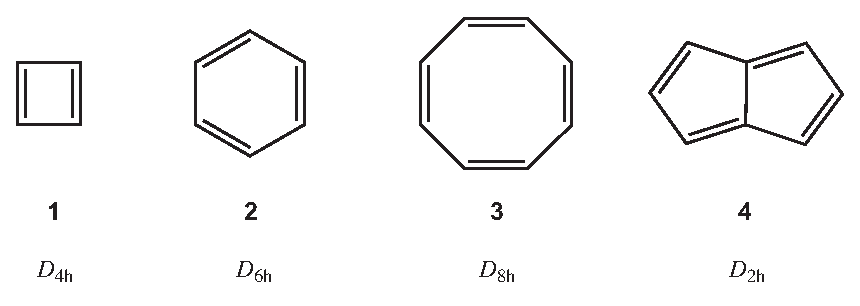
\includegraphics[scale=0.85]{orbopt/figures/compounds.eps}
\caption{Cyclobutadiene (\textbf{1}), benzene (\textbf{2}), cyclooctatetraene (\textbf{3}) and pentalene (\textbf{4}). Underneath the compound numbers the symmetry used for the respective compounds has been printed.}
\label{ch2.fig.compounds}
\end{figure}

Prior to any VB calculation, the geometry of the compounds had been optimized in the symmetry indicated in Figure \ref{ch2.fig.compounds}, using Restricted Hartree-Fock (RHF) with the \mbox{6-31G} basis set \cite{631g1,631g2}. The Valence Bond calculations, three per molecule, using the \textit{superci}, \textit{pert} and \textit{fock} options, were performed using delocalized $\sigma$ orbitals and strictly atomic $\pi$ orbitals, generated by a RHF calculation and an atomic SCF, respectively, all in the 6-31G basis. For all VB calculations, the DIIS option was switched on from the start. TURTLE's \textit{hybrid} option was used to separate the $\pi$ orbitals from each other and the $\sigma$ core. \textit{All} excitations were treated with perturbation, both for \textit{pert} and for \textit{fock}. In this case the \textit{fock} option can be used for the doubly occupied orbitals in the $\sigma$ core, because of the orthogonality of the $\pi$ orbitals to the $\sigma$ core. 

In Table \ref{ch2.tab.flat1} and \ref{ch2.tab.flat2} the results are presented. The total energies, presented below the name of each compound in the tables, was equal for all optimization methods for the first eight decimal places. Beneath the energies, for all methods the number of iterations, the total timings and the speed-up factors compared to regular Super CI are presented. In the case of the \textit{fock} option only the orbitals from the $\sigma$ core are optimized using the Fock algorithm; the $\pi$ orbitals are optimized using the \textit{pert} option in that case.

\begin{table}[htbp]
\caption{The total energy of both molecules ($E_{tot}$) is presented. The number of iterations, timing per iteration and speed-up factors (compared to \textit{superci}) for butadiene and benzene.}
\begin{center}
\begin{tabular}{l c c c c c c}
\hline
&\multicolumn{3}{c}{\textbf{Butadiene}}&\multicolumn{3}{c}{\textbf{Benzene}}\\
$E_{tot}$&\multicolumn{3}{c}{-153.59682368 au}&\multicolumn{3}{c}{-230.54408700 au}\\
\textbf{Method}&\textbf{\# iter}&\textbf{sec/iter}&\textbf{speed-up}&\textbf{\# iter}&\textbf{sec/iter}&\textbf{speed-up}\\
\hline
\textit{superci}&8&73.0&1&8&2274.1&1\\
\textit{pert}&14&4.9&8&13&90.8&15\\
\textit{fock}&10&4.8&12&10&79.3&23\\
\end{tabular}
\label{ch2.tab.flat1}
\end{center}
\end{table}

\begin{table}[htbp]
\caption{The total energy of both molecules ($E_{tot}$) is presented. The number of iterations, timing per iteration and speed-up factors (compared to \textit{superci}) for cyclooctatetraene and pentalene.}
\begin{center}
\begin{tabular}{l c c c c c c}
\hline
&\multicolumn{3}{c}{\textbf{Cyclooctatetraene}}&\multicolumn{3}{c}{\textbf{Pentalene}}\\
$E_{tot}$&\multicolumn{3}{c}{-307.35606250 au}&\multicolumn{3}{c}{-306.14034868 au}\\
\textbf{Method}&\textbf{\# iter}&\textbf{sec/iter}&\textbf{speed-up}&\textbf{\# iter}&\textbf{sec/iter}&\textbf{speed-up}\\
\hline
\textit{superci}&8&320106.0&1&8&47692.8&1\\
\textit{pert}&13&4704.2&42&14&1982.4&14\\
\textit{fock}&10&3857.0&66&12&1386.8&23\\
\end{tabular}
\label{ch2.tab.flat2}
\end{center}
\end{table}

For all molecules, the Super CI calculations take 8 iterations. Both in the \textit{fock} and in the \textit{pert} calculations more iterations are necessary to reach convergence. The approximation of the diagonal matrix element (Section \ref{ch2.sec.denominator}) seems to be beneficial for the calculation, because the number of iterations for \textit{fock} is smaller than for \textit{pert} in all four situations.

From the timings, it becomes clear that the \textit{fock} option is fruitful for this type of molecule, because the speed-up lies between 12 times for butadiene to 66 times for cyclooctatetraene compared to traditional Super CI. The difference between the speed-up of \textit{fock} and \textit{pert} is reasonable, but not as impressive as the difference between \textit{pert} and \textit{superci}. A drawback of the \textit{fock} option is the orthogonality condition that has to be met. 

Delocal VBSCF calculations, for which no examples have been presented here, do not suffer from this drawback, because in those calculations the doubly occupied orbitals will be orthogonal to each other, to the variably occupied orbitals and to the virtuals. However, most VB calculations in this thesis have been run with the \textit{hybrid} option, for which the \textit{fock} option is restricted to special cases, where the different \textit{hybrids} are orthogonal by symmetry.

\subsection{\label{ch2.sec.cyclopent}Second Example: The Cp-SiH Molecule}

For the work described in Chapter \chcyclopentadienyl\, a number of local VBSCF calculations have been performed to investigate the bonding mechanism of main group metal hydrides to cyclopentadienyl moieties. For details on the geometry optimization and the basis sets used, see Chapter \chcyclopentadienyl\ and reference \cite{budzelaar}. One of the molecules from that research is taken, the $\sigma$ bound \mbox{Cp-SiH} structure (Figure \ref{fig.cpsih}).
\begin{figure}[htdp]
\center
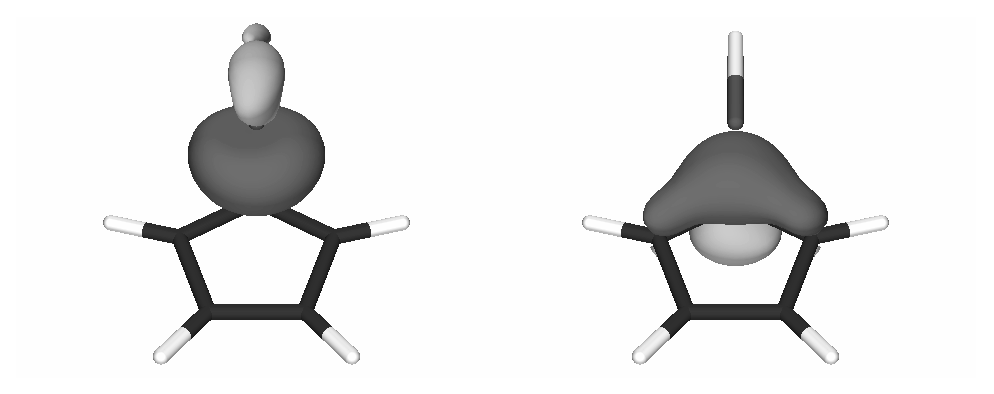
\includegraphics[scale=0.6]{orbopt/figures/sigma_sih.eps}
\caption{The $\sigma$ bound structure of Cp-SiH. Shown are the two singly occupied orbitals: the $sp$ hybridized orbital on SiH (left) and a $p$ orbital on the Cp-ring (right).}
\label{fig.cpsih}
\end{figure}
The calculation on this molecule forms a useful example for testing the additions to the optimization options, because the VBSCF process changes the orbitals drastically (in this case the total energy drops 0.86 Hartree between the initial and the final iteration). This is caused by the quality of the guess orbitals of which several are generated by hand instead of by a preceding Hartree-Fock calculation.

The molecule consists of two separate fragments, or \textit{hybrids} as they are referred to in TURTLE, \textit{i.e}, the cyclopentadienyl part and the siliconhydride part. In these parts the doubly occupied orbitals are orthogonal to each other, to the variably occupied and virtual orbitals inside their \textit{hybrid}. However, the \textit{hybrids} are not necessarily orthogonal to one another. In this case the orbitals in the cyclopentadienyl \textit{hybrid} are not orthogonal to the orbitals in the siliconhydride \textit{hybrid} and therefore the \textit{fock} option cannot be used.

For the original calculations TURTLE's \textit{super} option, which ensures that only excitations to virtual (unoccupied) orbitals are included in Super CI, was used. Without the \textit{super} option excitations to partly occupied orbitals are included as well. The reason was that the excitations from occupied orbitals in one structure to a partly vacant orbital in the same or in an other structure resulted in convergence problems. For the specification of the \textit{pert} option via orbital classes, this means that only excitations from doubly to unoccupied orbitals \mbox{(doc-uoc)} and excitations from variably to unoccupied orbitals \mbox{(voc-uoc)} have to be tested, since excitations from doubly occupied to variably occupied \mbox{(doc-voc)} and from variably to variably occupied orbitals \mbox{(voc-voc)} are not used in this \textit{super} VBSCF calculation.

Besides the effect of the \textit{pert} option, the effect of the convergence helpers DIIS \cite{diis1,diis2} and level shifting \cite{level1,level2} was analyzed. In DIIS a successive set of iterations, of which each has an associated set of new orbitals and a gradient vector ($\mathbf{b}$), are used to guess the new orbitals. For more details and its use in TURTLE, see appendix III in \cite{koos1}. With the level shifter in TURTLE, the value of $\left < \Psi_0 | \mathbf{H} - E_0 | \Psi_0 \right >$ is lowered by a user specified amount during the diagonalization step. A useful value for the shifter, if any, is found by trial and error. DIIS, when applied, was used from the first iteration on. For the level shifter, when applied, only the value 1 was used. This means that 1 au is subtracted from the upper left corner element in the Brillouin matrix, $\left< \Psi_0 | \mathbf{H} - E_0 | \Psi_0 \right>$. Furthermore, the convergence criterion was set to 1*10$^{-4}$ as maximum value for any of the Brillouin coefficients ($b_{ia}$, equation \ref{ch2.eq.superci}). This resulted in a total VB-energy which was, up to 5 decimal places, the same for all (converged) calculations: -481.44177 Hartree.

The results of the calculations are presented in Table \ref{ch2.tab.budzelaar}.
\begin{table}[htdp]
\caption{Timings in seconds of the VBSCF calculations on Cp-SiH (with the number of iterations between parenthesis). Three different optimization types were tested, regular Super CI, \textit{pert} doc-uoc and \textit{pert} doc-uoc/voc-uoc. With these different optimization types a combination of two convergence aids, DIIS and a level shifter (only for the \textit{pert} calculations) have been applied.}
\begin{center}
\begin{tabular}{l c c}
\hline
Type & no DIIS & DIIS \\
\hline
\textit{superci} & 3349 (11) & 2735 (9) \\ 
\textit{pert} doc-uoc & 1368 (99) & 324 (23)\\ 
\textit{pert} doc-uoc/voc-uoc & 1172 (98) & 316 (26)\\
\end{tabular}
\label{ch2.tab.budzelaar}
\end{center}
\end{table}
Without the convergence aid of a level shifter the calculations on this molecule with the \textit{pert} option switched on did not converge, while the regular Super CI calculation converged successfully in 11 iterations after 3349 seconds. Although the number of iterations needed to reach convergence is much larger than for a Super CI calculation, the total timings for the calculations with the \textit{pert} option are significantly lower. This is because the number of matrix elements necessary for \textit{pert} is much lower and therefore each iteration takes less time, but on the other hand information is discarded by leaving out matrix elements which results in (much) more iterations. 

Switching on DIIS appeared to be very beneficial for the \textit{pert} calculations, since it reduced the number of iterations roughly by a factor of four (Table \ref{ch2.tab.budzelaar}). For the \textit{superci} calculation DIIS was also advantageous: the calculation was shortened by almost 20\%.

\section{Conclusions}

Fock matrix elements, which can be calculated faster than Brillouin matrix elements, can be used for all excitations for which the orbital from which the excitation takes place (usually the doubly occupieds) and the orbital to which the excitation is, are orthogonal to each other and to the other orbitals. The other orbitals are allowed to be non-orthogonal to one another. In combination with the \textit{hybrid} option the \textit{fock} option can only be used when the doubly occupied orbitals in different \textit{hybrids} are orthogonal to all other orbitals.

When Fock matrix elements can be used, the calculation takes less time with the \textit{fock} than with the \textit{pert} option. However, the difference between \textit{fock} and \textit{pert} is not as impressive as the difference between \textit{pert} or \textit{fock} and \textit{superci}. Furthermore, the \textit{fock} option is not as generally applicable as the \textit{pert} option, because the latter does not require any orthogonality amongst the orbitals.

\section{Outlook}

In the theory section it has been shown that Brillouin matrix elements of the type $t \rightarrow a$ can be calculated from a series of inactive Fock matrix elements $F^{I}_{ta}$ and a set of second order cofactors (equation \ref{ch2.eq.ta_i7}). Although not implemented yet, computation time could be saved once it would be available in TURTLE. In that case, the construction of two separate Fock matrices is needed, $F^{I}_{ta}$ (for the inactive, or doubly occupied orbitals) and $F^{A}_{ta}$ (for the active, or variably occupied orbitals).

\section*{Appendix A: Cofactors}

A cofactor is a signed minor \cite{aitken}. A minor is created by removing one or more rows and columns from a determinant. Minors have the same sign as the original determinant from which they are derived. For a cofactor the sign depends on the position of the deleted row and column \cite{fokkeproef}. In this chapter the orbital overlap determinant, from which no rows and columns are removed, will be referred to as zeroth order cofactor. For a first order cofactor, obtained by removing one row and one column from the original determinant, the sign is $-1^{x+y}$, in which $x$ and $y$ are the indexes of the deleted row and column. For a second order cofactor, obtained by removing two rows and two columns from the original determinant, the sign is $-1^{x_1+x_2+y_1+y_2}$, in which $x_1$, $x_2$, $y_1$ and $y_2$ are the indexes of the deleted rows and columns. 

The overlap between two determinants can be expressed as  a zeroth order cofactor. The overlap of $\Delta_{1} = |ijkl \cdots n|$ with $\Delta_{2} = |ajkl \cdots n|$ for normalized orbitals is, \textit{e.g.}:
\begin{equation}
S_{12}^{(0)}=
\begin{array}{lllllll}
 &  i & j & k & l & \cdots & n \\
 a &  \multicolumn{1}{|l}{s_{ia}} & s_{ja}  & s_{ka} & s_{la} & & \multicolumn{1}{l|}{ s_{na} } \\
 j & \multicolumn{1}{|l}{s_{ij}} & 1 & s_{kj} & s_{lj} & & \multicolumn{1}{l|}{s_{nj}} \\
 k & \multicolumn{1}{|l}{s_{ik}} & s_{jk} & 1 & s_{lk} & & \multicolumn{1}{l|}{s_{nk}} \\
 l & \multicolumn{1}{|l}{s_{il}} & s_{jl} & s_{kl} & 1 & & \multicolumn{1}{l|}{s_{nl}} \\
 \vdots & \multicolumn{1}{|l}{ } &   &   & & \ddots & \multicolumn{1}{l|}{\vdots} \\
 n & \multicolumn{1}{|l}{ s_{in}} & s_{jn} & s_{kn} & s_{ln} & \cdots & \multicolumn{1}{l|}{1}
\end{array},\\
\label{ch2.eq.zocofac}
\end{equation}
in which the $s_{xy}$ elements stand for the orbital overlaps, \textit{i.e.} $\left < x | y \right >$. Along the rows and columns orbital labels are shown for readability. In the notation $S_{12}^{(0)}$, the superscript $(0)$ indicates that this is a zeroth order cofactor. The subscript $12$ indicates that the cofactor is constructed from overlaps of orbitals in determinant $\Delta_1$ with those from determinant $\Delta_2$.

A first order cofactor is derived from the zeroth order cofactor by removing one row and one column. So, when the column labeled $i$ and the row labeled $a$ are removed, the first order cofactor $S_{12}^{(i,a)}$ emerges:
\begin{equation}
S_{12}^{(i,a)} =
\begin{array}{lllllll}
 &  \hskip 2.0 pt \hbox{\lower 120pt\hbox{\vrule height128pt width 1.0pt}}\hskip-3.0pt i & j & k & l & \cdots & n \\
\noalign{\vskip-115pt}
 a &  \multicolumn{1}{|l}{s_{ia}} & s_{ja}  & s_{ka} & s_{la} & & \multicolumn{1}{l|}{ s_{na} } \\
\noalign{\vskip-8pt}
\multispan7\hbox{\vrule  height 1.0 pt width164pt}\cr
\noalign{\vskip 7pt}
  j & \multicolumn{1}{|l}{s_{ij}} & 1 & s_{kj} & s_{lj} & & \multicolumn{1}{l|}{s_{nj}} \\
 k & \multicolumn{1}{|l}{s_{ik}} & s_{jk} & 1 & s_{lk} & & \multicolumn{1}{l|}{s_{nk}} \\
 l & \multicolumn{1}{|l}{s_{il}} & s_{jl} & s_{kl} & 1 & & \multicolumn{1}{l|}{s_{nl}} \\
 \vdots & \multicolumn{1}{|l}{ } &   &   & & \ddots & \multicolumn{1}{l|}{\vdots} \\
 n & \multicolumn{1}{|l}{ s_{in}} & s_{jn} & s_{kn} & s_{ln} & \cdots & \multicolumn{1}{l|}{1}
\end{array}.\\
\label{ch2.eq.focofac}
\end{equation}
Since orbital $i$ is in the first column and orbital $a$ on the first row, the sign of the cofactor does not change because $-1^{(1+1)} = +1$.

When the columns labeled $i$ and $k$ and the rows labeled $a$ and $l$ are removed from $S_{12}^{(0)}$ the second order cofactor $S_{12}^{(i,k,a,l)}$ is generated:
\begin{equation}
S_{12}^{(i,k,a,l)} =
\begin{array}{lllllll}
 &  \hskip 2.0 pt \hbox{\lower 120pt\hbox{\vrule height128pt width 1.0pt}}\hskip-3.0pt i & j & \hskip 2.0 pt \hbox{\lower 120pt\hbox{\vrule height128pt width 1.0pt}}\hskip-3.0pt k & l & \cdots & n \\
\noalign{\vskip-115pt}
 a &  \multicolumn{1}{|l}{s_{ia}} & s_{ja}  & s_{ka} & s_{la} & & \multicolumn{1}{l|}{ s_{na} } \\
 \noalign{\vskip-8pt}
\multispan7\hbox{\vrule  height 1.0 pt width164pt}\cr
\noalign{\vskip 7pt}
 j & \multicolumn{1}{|l}{s_{ij}} & 1 & s_{kj} & s_{lj} & & \multicolumn{1}{l|}{s_{nj}} \\
 k & \multicolumn{1}{|l}{s_{ik}} & s_{jk} & 1 & s_{lk} & & \multicolumn{1}{l|}{s_{nk}} \\
 l & \multicolumn{1}{|l}{s_{il}} & s_{jl} & s_{kl} & 1 & & \multicolumn{1}{l|}{s_{nl}} \\
 \noalign{\vskip-8pt}
\multispan7\hbox{\vrule  height 1.0 pt width164pt}\cr
\noalign{\vskip 7pt}
 \vdots & \multicolumn{1}{|l}{ } &   &   & & \ddots & \multicolumn{1}{l|}{\vdots} \\
 n & \multicolumn{1}{|l}{ s_{in}} & s_{jn} & s_{kn} & s_{ln} & \cdots & \multicolumn{1}{l|}{1}
\end{array}.\\
\label{ch2.eq.socofac}
\end{equation}
In this second order cofactor the sign changes, because the position of the orbitals is: $i$ in the first and $k$ in the third column, $a$ on the first and $l$ on the fourth row. This makes $-1^{(1+3+1+4)} = -1$.

\bibliography{orbopt}
\bibliographystyle{../main/achemso}
